\chapter{Discrete Fourier Transform (DFT)}
We now discuss a powerful mathematical tool that can be approached from a least-square approximation viewpoint. In the last chapter, we have seen how to fit a polynomial curve to some data. It is then natural to ask further, whether there are other suitable types of curves that can be used for data fitting as well. Remember in Chapter \ref{chap:innerchap} we have derived the Fourier series which can expand any reasonable function in sines and cosines. Coincidentally, in the area of Earth Science, many phenomena can be described by the notion of \textit{waves}, which are often taken to be \textit{sinusoidal} during their derivation, e.g.\ atmospheric gravity waves, and seismic waves. However, in real life our sampling of data will be discrete. Therefore, we may want to know if we can do something similar and interpolate a discrete time-series by fitting sines and cosines to it, and this is the central idea of what is known as the \textit{Discrete Fourier Transform}.

\section{Mathematical Ideas of DFT}

\subsection{From Fourier Series to a Prototype of DFT}
\label{section:FouriertoDFT}

By Properties \ref{proper:fourierseries}, we know that any reasonable function $f(x)$ in the interval $[-\pi, \pi]$ can be written as 
\begin{align*}
f(x) = \frac{a_0}{2} + \sum_{m=1}^{\infty} a_m \cos(mx) + \sum_{n=1}^{\infty} b_n \sin(nx) 
\end{align*} where the Fourier coefficients $a_m$ and $b_n$ are given by Formulae (\ref{eqn:fouriera}) and (\ref{eqn:fourierb}). By a change of variable $x = \frac{2\pi}{N}t - \pi$, the interval is scaled to $t \in [0, N]$ where the cosines and sines are now in the form of
\begin{align*}
\cos(m(\frac{2\pi}{N}t - \pi)) &= \cos(\frac{2m\pi}{N}t) \\
\sin(n(\frac{2\pi}{N}t - \pi)) &= \sin(\frac{2n\pi}{N}t)
\end{align*}
The negative sign arising due to the $m\pi$ or $n\pi$ term inside is absorbed whenever needed. Since it involves a linear variable transformation only, these cosines and sines\footnote{\label{foot:fouriernorm} The normalization factor of $\sqrt{2/N}$ can be deduced by considering the squared norm of just the cosines themselves
\begin{align*}
\int_0^N \abs{\cos(\frac{2m\pi}{N}t)}^2 &= \int_0^N \frac{1}{2} (1+ \cos(\frac{4m\pi}{N}t)) dt \\
&= \frac{1}{2}(N) + (0) = \frac{N}{2}
\end{align*} and the same goes for the sines.} \begin{align*}
\left\{\sqrt{\frac{2}{N}}\sin(\frac{2\pi}{N}t), \sqrt{\frac{2}{N}}\sin(\frac{2\pi(2)}{N}t), \sqrt{\frac{2}{N}}\sin(\frac{2\pi(3)}{N}t), \ldots, \frac{1}{\sqrt{N}}, \right. \\ \left. \sqrt{\frac{2}{N}}\cos(\frac{2\pi}{N}t), \sqrt{\frac{2}{N}}\cos(\frac{2\pi(2)}{N}t), \sqrt{\frac{2}{N}}\cos(\frac{2\pi(3)}{N}t), \ldots \right\}    
\end{align*} are still an orthonormal basis to the new $L^2[0, N]$ space mapped from the initial $L^2[-\pi, \pi]$\footnote{Denote the original Fourier basis functions by $\varphi_j(x) \in L^2[-\pi, \pi]$. We will only show the part of linear independence and omit the justification for span and orthogonality. By Theorem \ref{thm:linearindep}, since they form a basis as given, $c_1\varphi_j(x) + c_2\varphi_j(x) + \cdots = 0(x) \equiv 0$ where $0(x)$ is the zero function, has the trivial solution $c_j = 0$ as its only solution. Assume the form of the linear change in variable is $x = \alpha t + \beta = X(t)$. Replacing $x$ by $X(t)$ (possible since $\alpha \neq 0$) then immediately produces the equality $c_1\varphi_j(X(t)) + c_2\varphi_j(X(t)) + \cdots = 0(X(t)) \equiv 0$ which automatically inherits the desired property of possessing only the trivial solution for the zero function as well and shows that the new basis functions are now $\hat{\varphi}_j(t) = \varphi_j(X(t))$.}. The Fourier coefficients are now computed by 
\begin{align}
a_m &= \frac{1}{\pi} \int_{-\pi}^{\pi} f(x)\cos(\frac{2m\pi}{N}t) d(\frac{2\pi}{N}t) = \frac{2}{N} \int_{0}^{N} f(t)\cos(\frac{2m\pi}{N}t) dt \label{eqn:fouriersca} \\
b_n &= \frac{1}{\pi} \int_{-\pi}^{\pi} f(x)\sin(\frac{2n\pi}{N}t) d(\frac{2\pi}{N}t) = \frac{2}{N} \int_{0}^{N} f(t)\sin(\frac{2n\pi}{N}t) dt \label{eqn:fourierscb}
\end{align}
where we have written $f(t)$ in place of $f(x) = f(\frac{2\pi}{N}t - \pi)$. The partial sum of the Fourier expansion of $f(t)$ up to degree $p$
\begin{align}
S_p(f(t)) &= \frac{a_0}{2} + \sum_{m=1}^{p} a_m \cos(\frac{2m\pi}{N}t) + \sum_{n=1}^{p} b_n \sin(\frac{2n\pi}{N}t) \label{eqn:fourierpart} \\
&= \frac{a_0}{2} + a_1 \cos(\frac{2\pi}{N}t) + a_2 \cos(\frac{2\pi(2)}{N}t) + \cdots + a_p \cos(\frac{2\pi p}{N}t) \nonumber \\
&\quad + b_1 \sin(\frac{2\pi}{N}t) + b_2 \sin(\frac{2\pi(2)}{N}t) + \cdots + b_p \sin(\frac{2\pi p}{N}t) \nonumber
\end{align}
will then be the best approximation of the function $f(t)$ using sines and cosines up to order $p$ with distance defined with respect to the inner product of Equation (\ref{eqn:integralinner}), a.k.a.\ the best-fit trigonometric polynomial of degree $p$. This is known as the \index{Best Approximation Theorem}\keywordhl{Best Approximation Theorem} which directly follows from Properties \ref{proper:shortestorthoproj}, in addition to the related discussion about orthogonal projections and the Fourier basis in Section \ref{section:orthoproj} because such a Fourier partial sum $S_p(f(t))$ is essentially an orthogonal projection of $f(t)$ onto the subspace spanned by the corresponding orthonormal trigonometric basis up to order $p$. Hence, the higher the degree of the partial sum of the Fourier expansion, the more closer the approximation to the given function. We use Example \ref{exmp:fourierx} as an illustration. The appropriate Fourier series of $x = f(t) = \frac{2\pi}{N}t - \pi$ is now
\begin{align*}
f(t) &= \sum_{n=1}^{\infty} b_n \sin(\frac{2n\pi}{N}t) \\
&= -2 \sum_{n=1}^{\infty} \frac{1}{n} \sin(\frac{2n\pi}{N}t)
\end{align*}
where $b_n = -\frac{2}{n}$. The following plot shows the original function as well as the partial sum of its Fourier expansion up to degree $3,10,20$. From this, we can see that as the degree $p$ goes up, $S_p(f(t))$ becomes a better approximation to the straight line $y = \frac{2\pi}{N}t - \pi$.\footnote{Notice that at the end-points, the values of Fourier series of $f(t) = \frac{2\pi}{N}t - \pi$ stay at $0$. It is because the Fourier series works as the periodic extension of the original function (see Footnote \ref{foot:fourier} in Chapter \ref{chap:innerchap}) and will converge to the average of the left and right limits $(f_-(t) + f_+(t))/2$ at point of discontinuity. Therefore, every end-point is essentially a discontinuity where one of the side limits is $\pi$ while the other is $-\pi$, so it converges to $((-\pi) + \pi)/2 = 0$.}\\
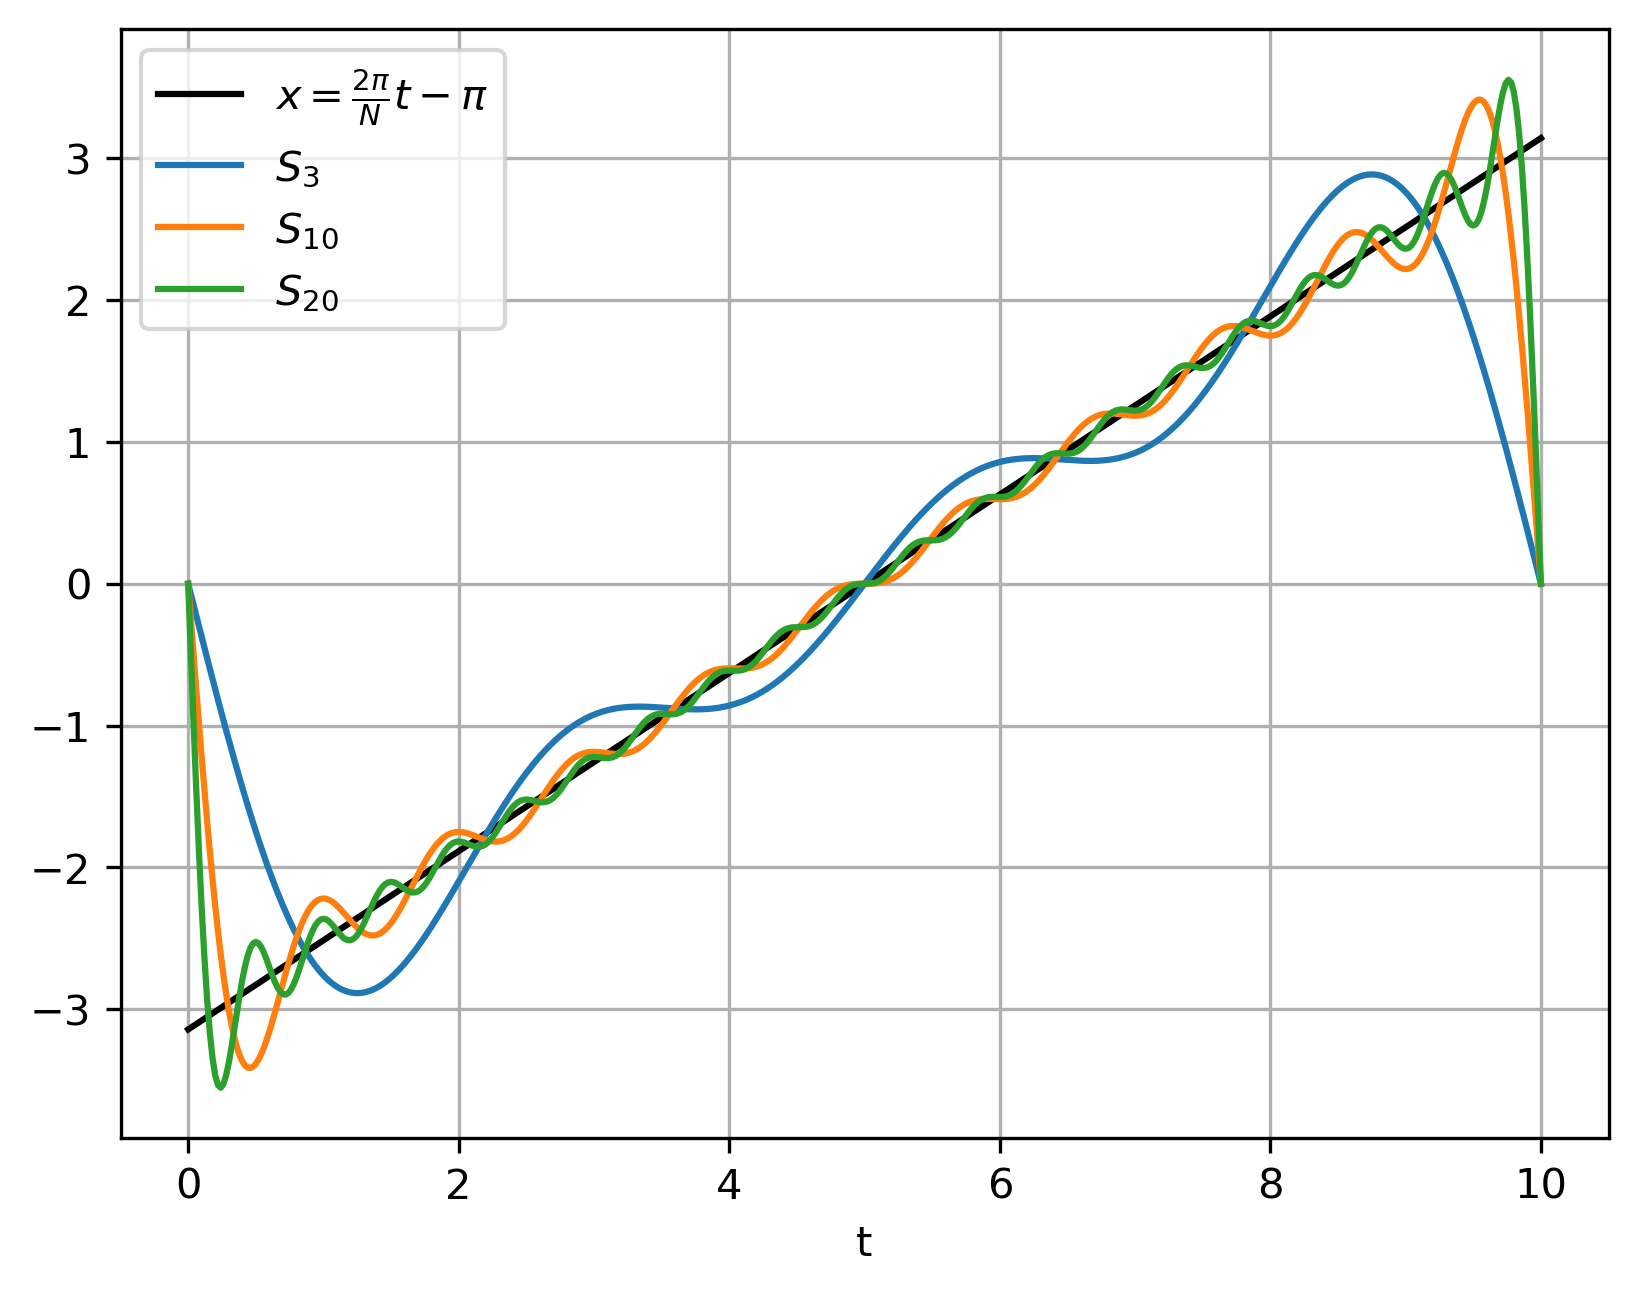
\includegraphics[scale=0.7]{graphics/fourierxapprox.png}\\
Eventually, as $p \to \infty$ and the expression tends to the full Fourier series, $S_p(f)$ will converge to $f$ in the $L^2$ sense\footnote{This is also called \textit{convergence in mean} and is different from \textit{pointwise convergence} that is more intuitive for most people. The rigorous treatment to this requires Measure Theory, and again, Functional Analysis and will not be pursued here.}, with respect to the inner product of Equation (\ref{eqn:integralinner}). To show this heuristically, we are going to derive the \textit{Bessel's Inequality} and \textit{Parseval's Identity} for a complete orthonormal basis in an $L^2$ space as below. (WIP, too messy, will be moved to Appendix) By part (d) of Theorem \ref{thm:spectralinner}, we can expand a function $f$ as
\begin{align*}
f = \lim_{p \to \infty} \sum_{j=1}^{p} \langle f, \varphi^{(j)} \rangle \varphi^{(j)} 
\end{align*}
where $\varphi^{(j)}$ are the orthonormal basis vectors/functions and the partial sum $S_p(f)$ will be just $\sum_{j=1}^{p} \langle f, \varphi^{(j)} \rangle \varphi^{(j)}$. Particularly, the completeness of the orthonormal basis in Properties \ref{proper:hilbertorthosys} means that (see the footnote below)\footnote{Otherwise, if $\norm{f - \sum_{j=1}^{\infty} \langle f, \varphi^{(j)} \rangle \varphi^{(j)}}^2 > 0$, then consider $\tilde{\varphi} = f - \sum_{j=1}^{\infty} \langle f, \varphi^{(j)} \rangle \varphi^{(j)}$ which is now a non-zero vector. It will be orthogonal to any of the original basis vectors $\varphi^{(j')}$ as 
\begin{align*}
\langle \tilde{\varphi}, \varphi^{(j')} \rangle &= \langle f - \sum_{j=1}^{\infty} \langle f, \varphi^{(j)} \rangle \varphi^{(j)} , \varphi^{(j')} \rangle \\
&= \langle f, \varphi^{(j')} \rangle - \langle \sum_{j=1}^{\infty} \langle f, \varphi^{(j)} \rangle \varphi^{(j)} , \varphi^{(j')} \rangle \\
&= \langle f, \varphi^{(j')} \rangle - (\cdots + (0) +\langle f, \varphi^{(j')} \rangle (1) + (0) + \cdots) \\
& \quad \text{(Orthonormality of the basis,} \\ 
& \quad \text{$\langle \varphi^{(j)}, \varphi^{(j')} \rangle = 1$ only when $j = j'$ and $0$ if $j \neq j'$.)} \\
&=\langle f, \varphi^{(j')} \rangle - \langle f, \varphi^{(j')} \rangle = 0
\end{align*}
which violates the premise of completeness as it will become another vector that is linearly independent of all the other basis vectors and can be added to the basis.}
\begin{align}
\norm{f - \sum_{j=1}^{\infty} \langle f, \varphi^{(j)} \rangle \varphi^{(j)}}^2 = 0 \label{eqn:fcomplete}
\end{align}
On the other hand,
\begin{align*} 
\norm{f - S_p(f)}^2 &= \norm{f - \sum_{j=1}^{p} \langle f, \varphi^{(j)} \rangle \varphi^{(j)}}^2 \\
&= \langle f - \sum_{j=1}^{p} \langle f, \varphi^{(j)} \rangle \varphi^{(j)}, f - \sum_{j=1}^{p} \langle f, \varphi^{(j)} \rangle \varphi^{(j)} \rangle \\
&= \langle f, f \rangle - \langle f, \sum_{j=1}^{p} \langle f, \varphi^{(j)} \rangle \varphi^{(j)} \rangle \\
&\quad - \langle \sum_{j=1}^{p} \langle f, \varphi^{(j)} \rangle \varphi^{(j)}, f \rangle \\
&\quad + \langle \sum_{j=1}^{p} \langle f, \varphi^{(j)} \rangle \varphi^{(j)}, \sum_{j=1}^{p} \langle f, \varphi^{(j)} \rangle \varphi^{(j)} \rangle \\
&= \norm{f}^2 - \langle f, \sum_{j=1}^{p} \langle f, \varphi^{(j)} \rangle \varphi^{(j)} \rangle \\
&\quad - \overline{\langle f, \sum_{j=1}^{p} \langle f, \varphi^{(j)} \rangle \varphi^{(j)} \rangle} \quad \text{(Definition \ref{defn:innerprod})} \\
&\quad + \sum_{j=1}^{p} \abs{\langle f, \varphi^{(j)} \rangle}^2 \quad \text{(Orthonormality of the basis)}\\
&= \norm{f}^2 - 2\Re{\langle f, \sum_{j=1}^{p} \langle f, \varphi^{(j)} \rangle \varphi^{(j)} \rangle} + \sum_{j=1}^{p} \abs{\langle f, \varphi^{(j)} \rangle}^2 \\
&= \norm{f}^2 - 2\Re{\sum_{j=1}^{p} (\overline{\langle f, \varphi^{(j)} \rangle} \langle f, \varphi^{(j)} \rangle)} \quad \text{(Properties \ref{proper:innerprod2})}\\
&\quad + \sum_{j=1}^{p} \abs{\langle f, \varphi^{(j)} \rangle}^2 \\
&= \norm{f}^2 - 2\sum_{j=1}^{p} \abs{\langle f, \varphi^{(j)} \rangle}^2 + \sum_{j=1}^{p} \abs{\langle f, \varphi^{(j)} \rangle}^2 \\
&= \norm{f}^2 - \sum_{j=1}^{p} \abs{\langle f, \varphi^{(j)} \rangle}^2
\end{align*}
and since $\norm{f - S_p(f)}^2 \geq 0$ is always non-negative, we have the \index{Bessel's Inequality}\keywordhl{Bessel's Inequality} as
\begin{align}
\sum_{j=1}^{p} \abs{\langle f, \varphi^{(j)} \rangle}^2 \leq \norm{f}^2  \label{eqn:Bessel}
\end{align}
From Exercise \ref{ex:triangular2}, we can apply the Triangular Inequality to get
\begin{align*}
&\norm{(f - \sum_{j=1}^{\infty} \langle f, \varphi^{(j)} \rangle \varphi^{(j)}) + (\sum_{j=1}^{\infty} \langle f, \varphi^{(j)} \rangle \varphi^{(j)} - S_p(f))}^2 \\
&= \norm{f - S_p(f)}^2 \leq \norm{f - \sum_{j=1}^{\infty} \langle f, \varphi^{(j)} \rangle \varphi^{(j)}}^2 + \norm{\sum_{j=1}^{\infty} \langle f, \varphi^{(j)} \rangle \varphi^{(j)} - S_p(f)}^2
\end{align*}
By Equation (\ref{eqn:fcomplete}), the first term on R.H.S. of the equality is zero. And the second term, when $p \to \infty$,
\begin{align*}
&\quad \norm{\sum_{j=1}^{\infty} \langle f, \varphi^{(j)} \rangle \varphi^{(j)} - S_p(f)}^2 \\
&= \norm{\sum_{j=p+1}^{\infty} \langle f, \varphi^{(j)} \rangle \varphi^{(j)}}^2 = \sum_{j=p+1}^{\infty} \abs{\langle f, \varphi^{(j)} \rangle}^2
\end{align*}
is a remainder term and must tend to zero, because $\sum_{j=1}^{p} \abs{\langle f, \varphi^{(j)} \rangle}^2$ is a convergent sequence, seen by applying the Monotone Convergence Theorem from elementary Analysis on Bessel's Inequality (\ref{eqn:Bessel}). Therefore, the L.H.S.
\begin{align*}
\lim_{p \to \infty}\norm{f - S_p(f)}^2 = 0
\end{align*}
also tends to zero as we take the same limit, which implies the $L^2$ convergence for a complete orthonormal basis, which includes the case of the Fourier series.\par
Returning to practices in Earth Science, and other fields like Engineering, often we are not given a function that has a closed form to work with. Instead, we collect data from measurements at a fixed sampling rate, and what we obtain is a \textit{discrete time series}. However, we can still try to apply the idea of Fourier, approximate and interpolate the finite time series with sinusoidal functions. Assume that, we have $N$ data points collected for the time series $f(t)$, evenly spaced at time $t = 0, 1, 2, \cdots, N-1$. Further assume that for now, we only use a few of sines and cosines for the approximation, such that the degree $p$ is much less than the number of data points $N$, specifically, $2p+1 \leq N$. The suitable Fourier approximation then will be in the form of Equation (\ref{eqn:fourierpart}) where $N$ is the period of the time series. Since we only have finite data points, we cannot carry out the needed integrations to compute (\ref{eqn:fouriersca}) and (\ref{eqn:fourierscb}). Nevertheless, we can borrow the idea in the last chapter and do the approximation in a way such that the Fourier partial sum will achieve the least-square error, summed over the sampling points. Subsequently, the system to be optimized will be
\begin{align*}
\footnotesize
\begin{cases}
\begin{aligned} 
C_0 + A_1 \cos(\frac{2\pi}{N}(0)) + A_2 \cos(\frac{2\pi(2)}{N}(0)) + \cdots + A_p \cos(\frac{2\pi p}{N}(0)) \\
+ B_1 \sin(\frac{2\pi}{N}(0)) + B_2 \sin(\frac{2\pi(2)}{N}(0)) + \cdots + B_p \sin(\frac{2\pi p}{N}(0))
\end{aligned} &= f(0) \\
\begin{aligned} 
C_0 + A_1 \cos(\frac{2\pi}{N}(1)) + A_2 \cos(\frac{2\pi(2)}{N}(1)) + \cdots + A_p \cos(\frac{2\pi p}{N}(1)) \\
+ B_1 \sin(\frac{2\pi}{N}(1)) + B_2 \sin(\frac{2\pi(2)}{N}(1)) + \cdots + B_p \sin(\frac{2\pi p}{N}(1))
\end{aligned} &= f(1) \\
\begin{aligned} 
C_0 + A_1 \cos(\frac{2\pi}{N}(2)) + A_2 \cos(\frac{2\pi(2)}{N}(2)) + \cdots + A_p \cos(\frac{2\pi p}{N}(2)) \\
+ B_1 \sin(\frac{2\pi}{N}(2)) + B_2 \sin(\frac{2\pi(2)}{N}(2)) + \cdots + B_p \sin(\frac{2\pi p}{N}(2))
\end{aligned} &= f(2) \\
\vdots \\
\begin{aligned} 
C_0 + A_1 \cos(\frac{2\pi}{N}(N-1)) + A_2 \cos(\frac{2\pi(2)}{N}(N-1)) + \cdots + A_p \cos(\frac{2\pi p}{N}(0)) \\
+ B_1 \sin(\frac{2\pi}{N}(N-1)) + B_2 \sin(\frac{2\pi(2)}{N}(N-1)) + \cdots + B_p \sin(\frac{2\pi p}{N}(N-1))
\end{aligned} &= f(N-1)
\end{cases}
\end{align*} 
where we have replaced the small letters $a_k, b_k$ by capital letters $A_k, B_k$ and $a_0$ by $C_0$. It can be expressed in the form of a matrix system, $G\vec{\beta} = \vec{d}$, where
\begin{align*}
G =
\small
\begin{bmatrix}
1 & 1 & 0 & \cdots & 1 & 0 \\
1 & \cos(\frac{2\pi}{N}) & \sin(\frac{2\pi}{N}) & \cdots & \cos(\frac{2\pi p}{N}) & \sin(\frac{2\pi p}{N}) \\
1 & \cos(\frac{2\pi(2)}{N}) & \sin(\frac{2\pi(2)}{N}) & \cdots & \cos(\frac{2\pi p (2)}{N}) & \sin(\frac{2\pi p (2)}{N}) \\
\vdots & \vdots & \vdots & & \vdots & \vdots \\
1 & \cos(\frac{2\pi(N-1)}{N}) & \sin(\frac{2\pi(N-1)}{N}) & \cdots & \cos(\frac{2\pi p(N-1)}{N}) & \sin(\frac{2\pi p(N-1)}{N}) \\
\end{bmatrix}
\end{align*}
is a $N \times (2p+1)$ matrix and
\begin{align*}
&\vec{\beta} = 
\begin{bmatrix}
C_0 \\
A_1 \\
B_1 \\
\vdots \\
A_p \\
B_p
\end{bmatrix}
&\vec{d} = 
\begin{bmatrix}
f(0) \\
f(1) \\
f(2) \\
\vdots \\
f(N-1)
\end{bmatrix}
\end{align*}
are vectors with $2p+1$ and $N$ entries respectively. The least-square method then sets out to find the best-fit parameters $\vec{\beta} = (C_0, A_1, B_1, \cdots, A_p, B_p)^T$ for this system of equations. From Theorem \ref{thm:bestfit}, we know that the best parameters are found by
\begin{align*}
\vec{\beta}_f = (G^TG)^{-1}G^T\vec{d}
\end{align*}
However, we can greatly simplify the expression, by noticing that every column vector of a sine/cosine series is orthogonal to each other. If we write each sine/cosine term as a complex exponential using Euler's formula in Definition \ref{defn:Euler}, then the column vectors of a sine-cosine pair in $G$ with a frequency of $2\pi k/N$, where both $k$ and $N$ are integers, can be expressed by the real and imaginary parts of
\begin{align*}
\left\{\exp(i \frac{2\pi k}{N} t)\right\}_{t = 0,1,2,\ldots,N-1}
&= \left\{\cos(\frac{2\pi k}{N} t) + i\sin(\frac{2\pi k}{N} t) \right\}_{t = 0,1,2,\ldots,N-1}
\end{align*}
or in the other way around,
\begin{align*}
\left\{\exp(-i \frac{2\pi k}{N} t)\right\}_{t = 0,1,2,\ldots,N-1}
&= \left\{\cos(\frac{2\pi k}{N} t) - i\sin(\frac{2\pi k}{N} t) \right\}_{t = 0,1,2,\ldots,N-1}
\end{align*}
We now first prove that the two column vectors of a sine-cosine pair that have the same frequency are orthogonal. We take the sum of squares of the first expression, which gives
\begin{align*}
\sum_{t=0}^{N-1} (\exp(i \frac{2\pi k}{N} t))^2 = \sum_{t=0}^{N-1} (\cos(\frac{2\pi k}{N} t) + i\sin(\frac{2\pi k}{N} t))^2 \\
\sum_{t=0}^{N-1} \exp(i \frac{4\pi k}{N} t) = \sum_{t=0}^{N-1} (\cos^2(\frac{2\pi k}{N} t) + 2i \sin(\frac{2\pi k}{N} t)\cos(\frac{2\pi k}{N} t) - \sin^2(\frac{2\pi k}{N} t))
\end{align*}
Notice that the left-hand side is a geometric sequence with a common ratio $r = \exp(\imath 4\pi k/N)$\footnote{which will not be equal to $1$ as we have demanded that $k \leq \frac{N-1}{2}$}, whose sum is seen to be
\begin{align*}
\frac{1-r^N}{1-r} &= \frac{1 - \exp(i 4\pi k)}{1 - \exp(i 4\pi k/N)} = 0
\end{align*}
as $\exp(\imath 4\pi k)$ is just $1$. By comparing the real and imaginary parts, we know that
\begin{align}
\sum_{t=0}^{N-1} \cos^2(\frac{2\pi k}{N} t) &= \sum_{t=0}^{N-1} \sin^2(\frac{2\pi k}{N} t) \label{eqn:sumofsincossq} \\
\sum_{t=0}^{N-1} \sin(\frac{2\pi k}{N} t)\cos(\frac{2\pi k}{N} t) &= 0
\end{align}
The second equation shows that the two column vectors representing the sine and cosine waves of the same frequency have a dot product of zero and hence are orthogonal. \par 

Utilizing the complex formulations, we can also prove that column vectors of sine (or cosine) functions with different frequencies are orthogonal as well. Here we prove one of the cases, where the first series is a sine with a frequency of $2\pi k/N$, and the second series is also a sine, of a frequency of $2\pi l/N$, where $k \neq l$ are both integers. We start by considering the sum of products between
\begin{align*}
\left\{\exp(i \frac{2\pi k}{N} t)\right\}_{t = 0,1,2,\ldots,N-1} = \left\{\cos(\frac{2\pi k}{N} t) + i\sin(\frac{2\pi k}{N} t) \right\}_{t = 0,1,2,\ldots,N-1} 
\end{align*}
and
\begin{align*}
\left\{\exp(i \frac{2\pi l}{N} t)\right\}_{t = 0,1,2,\ldots,N-1} = \left\{\cos(\frac{2\pi l}{N} t) + i\sin(\frac{2\pi l}{N} t) \right\}_{t = 0,1,2,\ldots,N-1} 
\end{align*}
The analysis is similar to the one above. Particularly, the L.H.S. is zero and by considering the real part of the expression on R.H.S., we have
\begin{align}
\sum_{t=0}^{N-1} \cos(\frac{2\pi k}{N} t)\cos(\frac{2\pi l}{N} t) - \sum_{t=0}^{N-1} \sin(\frac{2\pi k}{N} t)\sin(\frac{2\pi l}{N} t) &= 0 \label{eqn:cossinmixed1}
\end{align}
as long as $k + l$ is not the integer multiples of $N$. (why?)\footnote{The sum of complex exponentials on L.H.S. will then become
\begin{align*}
\sum_{t=0}^{N-1} \exp(i \frac{2\pi k}{N} t) \exp(i \frac{2\pi l}{N} t) &= \sum_{t=0}^{N-1} \exp(i \frac{2\pi k}{N} t) \exp(i \frac{2\pi (qN - k)}{N} t) \\
&= \sum_{t=0}^{N-1} \exp(i 2\pi q t) = \sum_{t=0}^{N-1} 1 = N \neq 0
\end{align*}
and the argument fails.} We can also consider another sum of products between $\left\{\exp(i \frac{2\pi k}{N} t)\right\}_{t = 0,1,2,\ldots,N-1}$ and
\begin{align*}
\left[\exp(-i \frac{2\pi l}{N} t)\right]_{t = 0,1,2,\cdots,N-1} = \left[\cos(\frac{2\pi l}{N} t) - i\sin(\frac{2\pi l}{N} t) \right]_{t = 0,1,2,\cdots,N-1}       
\end{align*}
Again by looking at the real part, this yields another relation as\footnote{Similarly we have the constraint that $k$ and $l$ are not differed by an integer multiple of $N$.}
\begin{align}
\sum_{t=0}^{N-1} \cos(\frac{2\pi k}{N} t)\cos(\frac{2\pi l}{N} t) + \sum_{t=0}^{N-1} \sin(\frac{2\pi k}{N} t)\sin(\frac{2\pi l}{N} t) &= 0 \label{eqn:cossinmixed2}
\end{align}
From the two derived equations (\ref{eqn:cossinmixed1}) and (\ref{eqn:cossinmixed2}), we can hence conclude that
\begin{align*}
\sum_{t=0}^{N-1} \cos(\frac{2\pi k}{N} t)\cos(\frac{2\pi l}{N} t) &= 0 \\
\sum_{t=0}^{N-1} \sin(\frac{2\pi k}{N} t)\sin(\frac{2\pi l}{N} t) &= 0        
\end{align*}
The orthogonality relations can be proven between sine and cosine of different frequencies as well in a very similar essence. We will now establish the last result, the dot product of any cosine (or sine) column vector with a specific frequency $2\pi k/N$ with itself. We can consider the sum of products between
\begin{align*}
&\left\{\exp(i\frac{2\pi k}{N} t)\right\}_{t = 0,1,2,\ldots,N-1} & \text{ and } & &\left\{\exp(-i \frac{2\pi k}{N} t)\right\}_{t = 0,1,2,\ldots,N-1}
\end{align*} 
This time, the L.H.S. is not a geometric series, but rather $N$ terms of $1$. The relation is then
\begin{align}
\sum_{t=0}^{N-1} \cos^2(\frac{2\pi k}{N} t) + \sum_{t=0}^{N-1} \sin^2(\frac{2\pi k}{N} t) &= \sum_{t=0}^{N-1} \exp(i \frac{2\pi k}{N} t)\exp(-i \frac{2\pi k}{N} t) \nonumber \\
&= \sum_{t=0}^{N-1} (1) \nonumber \\
&= N \label{eqn:samefreqcossin}
\end{align}
Actually, it can also be observed from the fact that the sum of a sine-cosine square pair is $1$. Not long before, we have arrived at Equation (\ref{eqn:sumofsincossq})
\begin{align*}
\sum_{t=0}^{N-1} \cos^2(\frac{2\pi k}{N} t) &= \sum_{t=0}^{N-1} \sin^2(\frac{2\pi k}{N} t)     
\end{align*}
Solving these two equations (\ref{eqn:sumofsincossq}) and (\ref{eqn:samefreqcossin}) yields
\begin{align}
\sum_{t=0}^{N-1} \cos^2(\frac{2\pi k}{N} t) &= \sum_{t=0}^{N-1} \sin^2(\frac{2\pi k}{n} t) = \frac{N}{2} \label{eqn:sqcossineNhalf}   
\end{align}
Hence the product $G^TG$, where each entry will be the dot product between the series of sines and cosines, will be
\begin{align*}
G^TG =
\begin{bmatrix}
N & 0 & 0 & \cdots \\
0 & \frac{N}{2} & 0 & \\
0 & 0 & \frac{N}{2} & \\
\vdots & & & \ddots
\end{bmatrix}
\end{align*}
and
\begin{align*}
(G^TG)^{-1} = \frac{1}{N}
\begin{bmatrix}
1 & 0 & 0 & \cdots \\
0 & 2 & 0 & \\
0 & 0 & 2 & \\
\vdots & & & \ddots
\end{bmatrix}    
\end{align*}
So the best-fit parameters are
\begin{align*}
\vec{\beta_f} &= (G^TG)^{-1}G^T\vec{d} \\
\begin{bmatrix}
C_0 \\
A_1 \\
B_1 \\
\vdots \\
\end{bmatrix}
&= \frac{1}{N} 
\begin{bmatrix}
1 & 0 & 0 & \cdots \\
0 & 2 & 0 & \\
0 & 0 & 2 & \\
\vdots & & & \ddots
\end{bmatrix} 
\begin{bmatrix}
1 & 1 & 1 & \cdots \\
1 & \cos(\frac{2\pi}{N}) & \cos(\frac{2\pi(2)}{N}) & \\
0 & \sin(\frac{2\pi}{N}) & \sin(\frac{2\pi(2)}{N}) &  \\
\vdots & & & \ddots
\end{bmatrix}
\begin{bmatrix}
f(0)\\
f(1)\\
f(2)\\
\vdots
\end{bmatrix} \\
\begin{bmatrix}
C_0 \\
A_1 \\
B_1 \\
\vdots \\
\end{bmatrix}
&= 
\frac{1}{N}
\begin{bmatrix}
1 & 1 & 1 & \cdots \\
2 & 2\cos(\frac{2\pi}{N}) & 2\cos(\frac{2\pi(2)}{N}) & \\
0 & 2\sin(\frac{2\pi}{N}) & 2\sin(\frac{2\pi(2)}{N}) &  \\
\vdots & & & \ddots
\end{bmatrix}
\begin{bmatrix}
f(0)\\
f(1)\\
f(2)\\
\vdots
\end{bmatrix} 
\end{align*}
Detailed expressions are
\begin{align}
C_0 &= \frac{1}{N}(f(0) + f(1) + f(2) + \cdots + f(N-1)) \nonumber \\
&= \frac{1}{N}\sum_{t=0}^{n-1} f(t) \label{eqn:protoDFTc}  \\
A_k &= \frac{2}{N}(f(0) + f(1)\cos(\frac{2\pi k}{N}) + \cdots + f(N-1)\cos(\frac{2\pi k(N-1)}{N})) \nonumber \\
&= \frac{2}{N}\sum_{t=0}^{N-1} f(t)\cos(\frac{2\pi kt}{N}) \label{eqn:protoDFTa} \\
B_k &= \frac{2}{N}(f(1)\sin(\frac{2\pi k}{N}) + \cdots + f(N-1)\sin(\frac{2\pi k (N-1)}{N})) \nonumber \\
&= \frac{2}{N}\sum_{t=0}^{N-1} f(t)\sin(\frac{2\pi kt}{N}) \label{eqn:protoDFTb}
\end{align}
That makes sense, at least they seem to be. But in the short exercise that follows the example below you will immediately notice that there is a big caveat to this prototype.
\begin{exmp}
\label{exmp:ex11.2.1}
Fit the following time-series with the Fourier basis up to order $p=1$, where $f(0) = 4, f(1) = 1, f(2) = 2, f(3) = 3, f(4) = 1$.
\end{exmp}
\begin{solution}
The degree is $p=1$ and it means that there are only three components, which are the constant term, and a sine-cosine pair with a frequency of $\frac{2\pi k}{N}$ where $k=1$, $N=5$. The best-fit parameters will be
\begin{align*}
\small
\begin{bmatrix}
C_0 \\
A_1 \\
B_1
\end{bmatrix}
&= 
\frac{1}{5}
\small
\begin{bmatrix}
1 & 1 & 1 & 1 & 1 \\
2 & 2\cos(\frac{2\pi}{5}) & 2\cos(\frac{2\pi(2)}{5}) & 2\cos(\frac{2\pi(3)}{5}) & 2\cos(\frac{2\pi(4)}{5}) \\
0 & 2\sin(\frac{2\pi}{5}) & 2\sin(\frac{2\pi(2)}{5}) & 2\sin(\frac{2\pi(3)}{5}) & 2\sin(\frac{2\pi(4)}{5})
\end{bmatrix}
\small
\begin{bmatrix}
f(0)\\
f(1)\\
f(2)\\
f(3)\\
f(4)
\end{bmatrix} 
\end{align*}
\begin{align*}
C_0 &= \frac{1}{5} (4+1+2+3+1) = \frac{11}{5} \\
A_1 &= \frac{2}{5} (4 + 1\cos(\frac{2\pi}{5}) + 2\cos(\frac{2\pi(2)}{5}) + 3\cos(\frac{2\pi(3)}{5}) + 1\cos(\frac{2\pi(4)}{5})) \\
&\approx 0.229 \\
B_1 &= \frac{2}{5} (0 + 1\sin(\frac{2\pi}{5}) + 2\sin(\frac{2\pi(2)}{5}) + 3\sin(\frac{2\pi(3)}{5}) + 1\sin(\frac{2\pi(4)}{5})) \\
&\approx -0.235
\end{align*}
So the best trigonometric fit of order $p=1$ for the time-series concerned is
\begin{align*}
f(t) = \frac{11}{5} + 0.229 \cos(\frac{2\pi}{5}t) - 0.235 \sin(\frac{2\pi}{5}t)
\end{align*}
\end{solution}
Short Exercise: Find an improved approximation with order $p = 2$. What happens if $p = 3$? \footnote{For $p = 2$, the best-fit coefficients are
\begin{align*}
\begin{bmatrix}
C_0 \\
A_1 \\
B_1 \\
A_2 \\
B_2
\end{bmatrix}
&= 
\frac{1}{5}
\begin{bmatrix}
1 & 1 & 1 & 1 & 1 \\
2 & 2\cos(\frac{2\pi}{5}) & 2\cos(\frac{2\pi(2)}{5}) & 2\cos(\frac{2\pi(3)}{5}) & 2\cos(\frac{2\pi(4)}{5}) \\
0 & 2\sin(\frac{2\pi}{5}) & 2\sin(\frac{2\pi(2)}{5}) & 2\sin(\frac{2\pi(3)}{5}) & 2\sin(\frac{2\pi(4)}{5}) \\
2 & 2\cos(\frac{2\pi(2)}{5}) & 2\cos(\frac{2\pi(2)(2)}{5}) & 2\cos(\frac{2\pi(2)(3)}{5}) & 2\cos(\frac{2\pi(2)(4)}{5}) \\
0 & 2\sin(\frac{2\pi(2)}{5}) & 2\sin(\frac{2\pi(2)(2)}{5}) & 2\sin(\frac{2\pi(2)(3)}{5}) & 2\sin(\frac{2\pi(2)(4)}{5})
\end{bmatrix}
\begin{bmatrix}
f(0)\\
f(1)\\
f(2)\\
f(3)\\
f(4)
\end{bmatrix}     
\end{align*}
It is not hard to see that $C_0, A_1, B_1$ will be the same and
\begin{align*}
A_2 &= \frac{2}{5} (4 + 1\cos(\frac{2\pi(2)}{5}) + 2\cos(\frac{2\pi(2)(2)}{5}) + 3\cos(\frac{2\pi(2)(3)}{5}) + 1\cos(\frac{2\pi(2)(4)}{5})) \\
&\approx 1.571 \\
B_2 &= \frac{2}{5} (0 + 1\sin(\frac{2\pi(2)}{5}) + 2\sin(\frac{2\pi(2)(2)}{5}) + 3\sin(\frac{2\pi(2)(3)}{5}) + 1\sin(\frac{2\pi(2)(4)}{5})) \\
&\approx 0.380
\end{align*}
Hence the new approximation will be $f(t) = \frac{11}{5} + 0.229 \cos(\frac{2\pi}{5}t) - 0.235 \sin(\frac{2\pi}{5}t) + 1.571 \cos(\frac{2\pi(2)}{5}t) + 0.380 \sin(\frac{2\pi(2)}{5}t)$. When $p$ is increased to $3$, the matrix $G$ involved in the best-fit formula becomes
\begin{align*}
\scriptsize
G = 
\begin{bmatrix}
1 & 1 & 0 & 1 & 0 & 1 & 0 \\
1 & \cos(\frac{2\pi}{5}) & \sin(\frac{2\pi}{5}) & \cos(\frac{2\pi(2)}{5}) & \sin(\frac{2\pi(2)}{5}) & \cos(\frac{2\pi(3)}{5}) & \sin(\frac{2\pi(3)}{5})\\
1 & \cos(\frac{2\pi(2)}{5}) & \sin(\frac{2\pi(2)}{5}) & \cos(\frac{2\pi(2)(2)}{5}) & \sin(\frac{2\pi(2)(2)}{5}) & \cos(\frac{2\pi(3)(2)}{5}) & \sin(\frac{2\pi(3)(2)}{5}) \\
1 & \cos(\frac{2\pi(3)}{5}) & \sin(\frac{2\pi(3)}{5}) & \cos(\frac{2\pi(2)(3)}{5}) & \sin(\frac{2\pi(2)(3)}{5}) & \cos(\frac{2\pi(3)(3)}{5}) & \sin(\frac{2\pi(3)(3)}{5})\\
1 & \cos(\frac{2\pi(4)}{5}) & \sin(\frac{2\pi(4)}{5}) & \cos(\frac{2\pi(2)(4)}{5}) & \sin(\frac{2\pi(2)(4)}{5}) & \cos(\frac{2\pi(3)(4)}{5}) & \sin(\frac{2\pi(3)(4)}{5})
\end{bmatrix}    
\end{align*}
\vspace{\maxdimen}
and a routine computation will show that
\begin{align*}
G^T G = 
\begin{bmatrix}
5 & 0 & 0 & 0 & 0 & 0 & 0 \\
0 & \frac{5}{2} & 0 & 0 & 0 & 0 & 0 \\
0 & 0 & \frac{5}{2} & 0 & 0 & 0 & 0 \\
0 & 0 & 0 & \frac{5}{2} & 0 & \frac{5}{2} & 0 \\
0 & 0 & 0 & 0 & \frac{5}{2} & 0 & -\frac{5}{2} \\
0 & 0 & 0 & \frac{5}{2} & 0 & \frac{5}{2} & 0 \\
0 & 0 & 0 & 0 & -\frac{5}{2} & 0 & \frac{5}{2} \\
\end{bmatrix}
\end{align*}
which is not invertible (the fourth/sixth rows are equal and the fifth/last rows are the negative of each other), so that the formula $\vec{\beta}_f = (G^TG)^{-1}G^T\vec{d}$ will fail. If we forcefully use the expressions in (\ref{eqn:protoDFTa}) and (\ref{eqn:protoDFTb}) to compute $A_3$ and $B_3$ we will get
\begin{align*}
A_3 &= \frac{2}{5} (4 + 1\cos(\frac{2\pi(3)}{5}) + 2\cos(\frac{2\pi(3)(2)}{5}) + 3\cos(\frac{2\pi(3)(3)}{5}) + 1\cos(\frac{2\pi(3)(4)}{5})) \\
&= A_2 \\
B_3 &= \frac{2}{5} (0 + 1\sin(\frac{2\pi(3)}{5}) + 2\sin(\frac{2\pi(3)(2)}{5}) + 3\sin(\frac{2\pi(3)(3)}{5}) + 1\sin(\frac{2\pi(3)(4)}{5})) \\
&= -B_2    
\end{align*}
So $A_2$ ($B_2$) and $A_3$ ($B_3$) carry the same information and one of them will be redundant.
}

\subsection{Nyquist Frequency and Real DFT}

While we may want to make the approximation by the Fourier basis as good as possible, we have to know how high the order $p$ needs to be. On the other hand, as we can see in the last example, if $p$ is set too large, the best-fit formula will become problematic and the approximation will contain duplicated terms, in the sense that they take equal values (or with an opposite sign) at all sampling points. For example, if $k + l = N$, then for the integer time steps $t = 0, 1, \ldots, N-1$
\begin{align*}
\cos(\frac{2\pi l}{N} t) &= \cos(\frac{2\pi (N-k)}{N} t) \\
&= \cos(2\pi t - \frac{2\pi k}{N} t) \\
&= \cos(\frac{2\pi k}{N} t)
\end{align*}
so the two cosine waves, despite having different frequencies, coincide at every data point and will be indistinguishable within the time-series. The same problem arises similarly for the sine terms. The condition $k + l = N$ above hints that the maximum value of $p$ should be $N/2$. This corresponds to an angular frequency of $\omega_{\text{Ny}} = \frac{2\pi}{N}(\frac{N}{2}) = \pi$, which is known as the \index{Nyquist Frequency}\keywordhl{Nyquist frequency}. Consequentially, we have the \index{Nyquist Sampling Theorem}\keywordhl{Nyquist Sampling Theorem} as follows.
\begin{thm}[Nyquist Sampling Theorem]
\label{thm:Nyquist}
For an evenly spaced time-series that has a time step of $\Delta t = 1$, any sinusoidal wave with an angular frequency exceeding the Nyquist frequency $\omega > \omega_{\text{Ny}} = \pi$ cannot be properly detected. 
\end{thm}
So it means that the highest resolvable frequency in the time-series is the Nyquist frequency $\omega_{\text{Ny}} = \pi$, or in other words, the minimum period length has to cover at least two time steps. As a result, we only need the sine/cosine terms up to the order $\lfloor N/2 \rfloor$. We have just shown a part of the theorem that if $k + l = N$, then the sinusoidal series of a higher order $l = \lfloor N/2 \rfloor + 1, \ldots, N$ will be redundant in the derivation above. We will complete the theorem by verifying that the sine/cosine terms of an order $l = N+1, N+2, \ldots$ beyond will also lead to duplicated modes: let $l = k + qN$ where $q$ is a positive integer, then
\begin{align*}
\cos(\frac{2\pi l}{N} t) &= \cos(\frac{2\pi (k + qN)}{N} t) \\
&= \cos(\frac{2\pi k}{N} t + 2\pi q t) \\
&= \cos(\frac{2\pi k}{N} t)
\end{align*}
for all time steps $t = 0,1,\ldots,N-1$. Again, it is similar for the sines. Another perspective to see the problem is that, if the "ground truth" function to be approximated by DFT indeed contains some sinusoidal component with a frequency higher than the Nyquist frequency, then its signal will "spill" into a corresponding lower frequency. Again, using cosine and the case $k + l = N$ as an illustration, if $k$ represents the lower frequency mode and $l$ represents the higher one (assumed to have a Fourier coefficient of $a_l$ in the "ground truth"), then (\ref{eqn:protoDFTa}) will yield
\begin{align*}
A_{k \leftarrow l} &= \frac{2}{N}\sum_{t=0}^{N-1} (a_l\cos(\frac{2\pi lt}{N})) \cos(\frac{2\pi kt}{N}) \\
&= \frac{2}{N}\sum_{t=0}^{N-1} a_l\cos(\frac{2\pi (N-k)t}{N}) \cos(\frac{2\pi kt}{N}) \\
&= \frac{2}{N}\sum_{t=0}^{N-1} a_l\cos(2\pi t - \frac{2\pi k}{N} t) \cos(\frac{2\pi kt}{N}) \\
&= \frac{2}{N}\sum_{t=0}^{N-1} a_l\cos(\frac{2\pi k}{N} t)) \cos(\frac{2\pi kt}{N}) \\
&= \frac{2}{N}\sum_{t=0}^{N-1} a_l \cos^2(\frac{2\pi kt}{N}) \\
&= \frac{2}{N} (a_l (\frac{N}{2})) = a_l & \text{(Equation (\ref{eqn:sqcossineNhalf}))} 
\end{align*}
Hence any signal with a frequency higher than the Nyquist frequency will contribute to the respective DFT frequency and contaminate it.\footnote{On the other hand, if the true function only contains the lower frequency mode, then by the same steps we can show that the prototype DFT coefficient $A_k$ will coincide exactly with the usual Fourier coefficients $a_k$.}\par

Now we can formally derive the \index{Real Discrete Fourier Transform}\keywordhl{(real) Discrete Fourier Transform} for a time-series which is given by (\ref{eqn:protoDFTc}), (\ref{eqn:protoDFTa}), and (\ref{eqn:protoDFTb}). In the last part, we have already worked with an odd $N$ (see Example \ref{exmp:ex11.2.1}) where the maximum resolvable degree will be $p = \frac{N}{2} - 1$. When $N$ is even, then we have frequencies from zero to $k = \frac{N}{2}$. Notice that the constant term of zero frequency contributes a single parameter, every other frequency contributes two coefficients via a pair of sine and cosine, and the maximum frequency $k_{\text{Ny}} = \frac{N}{2}$ only gives rise to one coefficient from the cosine series which takes the form of alternating $(1,-1,1,-1,\ldots,1,-1)$ (the corresponding diagonal entry in the $(G^TG)^{-1}$ term of the least-square formula will be $1/N$ instead of $2/N$), as the sine function will be always zero at the Nyquist frequency. In both cases, there can be at most $N$ sinusoidal curves for fitting $N$ data points and $G$ will be square. Since the amount of parameters is the same as the number of data, it becomes an interpolation that passes through all the given data points. By convention, we will omit the factor of $1/N$ in the computation of DFT.

\begin{exmp}
Find the Discrete Fourier Transform of the time series $(1,2,1,-1,3,0,2,-2)$.
\end{exmp}
\begin{solution}
According to Theorem \ref{thm:Nyquist}, the highest resolvable degree will be $N/2 = 4$. Its DFT is then given by
\begin{align*}
\scriptsize
\begin{bmatrix}
C_0 \\
A_1 \\
B_1 \\
A_2 \\
B_2 \\
A_3 \\
B_3 \\
A_4
\end{bmatrix}
&= 
\tiny
\begin{bmatrix}
1 & 1 & 1 & 1 & \cdots & 1 & 1 \\
2 & 2\cos(\frac{2\pi}{8}) & 2\cos(\frac{2\pi(2)}{8}) & 2\cos(\frac{2\pi(3)}{8}) & \cdots & 2\cos(\frac{2\pi(6)}{8}) & 2\cos(\frac{2\pi(7)}{8}) \\
0 & 2\sin(\frac{2\pi}{8}) & 2\sin(\frac{2\pi(2)}{8}) & 2\sin(\frac{2\pi(3)}{8}) & \cdots & 2\sin(\frac{2\pi(6)}{8}) & 2\sin(\frac{2\pi(7)}{8}) \\
2 & 2\cos(\frac{2\pi(2)}{8}) & 2\cos(\frac{2\pi(2)(2)}{8}) & 2\cos(\frac{2\pi(2)(3)}{8}) & \cdots & 2\cos(\frac{2\pi(2)(6)}{8}) & 2\cos(\frac{2\pi(2)(7)}{8}) \\
0 & 2\sin(\frac{2\pi(2)}{8}) & 2\sin(\frac{2\pi(2)(2)}{8}) & 2\sin(\frac{2\pi(2)(3)}{8}) & \cdots & 2\sin(\frac{2\pi(2)(6)}{8}) & 2\sin(\frac{2\pi(2)(7)}{8}) \\
2 & 2\cos(\frac{2\pi(3)}{8}) & 2\cos(\frac{2\pi(3)(2)}{8}) & 2\cos(\frac{2\pi(3)(3)}{8}) & \cdots & 2\cos(\frac{2\pi(3)(6)}{8}) & 2\cos(\frac{2\pi(3)(7)}{8}) \\
0 & 2\sin(\frac{2\pi(3)}{8}) & 2\sin(\frac{2\pi(3)(2)}{8}) & 2\sin(\frac{2\pi(3)(3)}{8}) & \cdots & 2\sin(\frac{2\pi(3)(6)}{8}) & 2\sin(\frac{2\pi(3)(7)}{8}) \\
1 & -1 & 1 & -1 & \cdots & 1 & -1
\end{bmatrix}
\scriptsize
\begin{bmatrix}
f(0)\\
f(1)\\
f(2)\\
f(3)\\
f(4)\\
f(5)\\
f(6)\\
f(7)
\end{bmatrix}     
\end{align*}
A direct computation then gives 
\begin{align*}
&\quad (C_0, A_1, B_1, A_2, B_2, A_3, B_3, A_4)^T \\
&= (6, -2.586, 2.243, 2, 10, -5.414, 6.243, 8)^T
\end{align*}
\end{solution}

\subsection{Complex DFT}

The real DFT approach above has the drawback of using sine-cosine pairs for computation. In Section \ref{section:complexno}, we have learned the power of complex exponentials to simultaneously represent sines and cosines through Euler's formula, which has also been exploited to derive the relationships between the sinusoidal functions when we are developing the DFT prototype. Therefore, it is incentive to explore the possibility of using complex exponentials to define Discrete Fourier Transform. This has the benefits of simplicity and also convenience when programming.

Continuing from the ideas built in the last section, we propose an interpolation scheme which uses $\exp(i (2\pi k/N) t)$, for a time-series with $N$ data, evenly spaced by a time step of $\Delta t = 1$. The range of $k$ will be from $-\frac{N}{2}, -(\frac{N}{2}-1), \ldots, -1, \allowbreak 0, 1, \ldots, \frac{N}{2}-1$ for even $N$ and $-\frac{N-1}{2}, -(\frac{N-1}{2}-1), \dots, -1, 0, 1, \ldots, \frac{N-1}{2}$ for odd $N$. Both ranges ensure that the total number of complex exponentials used in the fitting process is exactly $N$. Each pair of $k$ and $-k$, i.e.\ $\exp(i (2\pi k/N) t)$ and $\exp(-i (2\pi k/N) t)$ in combination, gives rise to $\cos(\frac{2\pi k}{N} t)$ and $\sin(\frac{2\pi k}{N} t)$ by Properties \ref{proper:sincoscomplex}, and so we can expect the correspondence between the real and complex version of Discrete Fourier Transform.\\
\\
Now, the matrix $G$ will take the form of
\begin{align*}
G = \tiny
\renewcommand\arraystretch{1.33}
\left[\begin{array}{@{\,}wc{5pt}wc{40pt}wc{40pt}wc{8pt}wc{56pt}wc{56pt}wc{8pt}wc{40pt}}
1 & 1 & 1 & \cdots & 1 & 1 & \cdots & 1\\
1 & \exp(\imath\frac{2\pi}{N}) & \exp(\imath\frac{2\pi(2)}{N}) & \cdots & \exp(\imath\frac{2\pi(\frac{N}{2}-1)}{N}) & \exp(\imath\frac{2\pi(-\frac{N}{2})}{N}) & \cdots & \exp(-\imath\frac{2\pi}{N}) \\
1 & \exp(\imath\frac{2\pi(2)}{N}) & \exp(\imath\frac{2\pi(2)(2)}{N}) & \cdots & \exp(\imath\frac{2\pi(\frac{N}{2}-1)(2)}{N}) & \exp(\imath\frac{2\pi(-\frac{N}{2})(2)}{N}) & \cdots & \exp(-\imath\frac{2\pi(2)}{N})\\
\vdots & \vdots & & \vdots & \vdots & \vdots &  & \\
1 & \exp(\imath\frac{2\pi(N-1)}{N}) & \exp(\imath\frac{2\pi(2)(N-1)}{N}) & \cdots & \exp(\imath\frac{2\pi(\frac{N}{2}-1)(N-1)}{N}) & \exp(\imath\frac{2\pi(-\frac{N}{2})(N-1)}{N}) & \cdots & \exp(-\imath\frac{2\pi(N-1)}{N}) \\
\end{array}\right]
\end{align*}
for even $N$, where each column represents frequencies corresponding to $k = 0, 1, \ldots, \frac{N}{2}-1, -\frac{N}{2}, \ldots, -1$. This is a common convention where we start from $k = 0$, and it increases to the largest positive $k = \frac{N}{2}-1$, then we flip the sign and resume from the most negative $k = -\frac{N}{2}$, finally go all the way back to $k = -1$. For odd $N$, the matrix $G$ is essentially the same, except the $k$ is replaced by the appropriate range of integers, and in particular the flipping leads to $k = -\frac{N-1}{2}$ from $k = \frac{N-1}{2}$. \par
The entries of $G^*G$ in the formula from Theorem \ref{thm:bestfit} are then the complex dot products between the sequences of complex exponentials appearing as the column vectors of $G$. The orthogonality relation between different column vectors of $G$ is very easy to find. The procedure is similar to what we have done when proving the orthogonality for the real case, but even less tedious. The key point is to write the complex dot product over any pair of two columns as a geometric sequence, that when the values of $k$ are different, will be evaluated to zero. The readers are invited to verify this result, in addition to the fact that the complex dot product between any such a column vector and itself is $N$.\footnote{When $k \neq l$, we have \begin{align*}
\sum_{t=0}^{N-1} \exp(i (2\pi k/N) t)\overline{\exp(i (2\pi l/N) t)} &= \sum_{t=0}^{N-1} \exp(i (2\pi k/N) t)\exp(-i (2\pi l/N) t) \\
&= \sum_{t=0}^{N-1} \exp(i (2\pi (k-l)/N) t) \\
&= \frac{1-\exp(i (2\pi (k-l)/N))^N}{1-\exp(i (2\pi (k-l)/N))} \\
&= \frac{1-\exp(i (2\pi (k-l)))}{1-\exp(i (2\pi (k-l)/N))} \\
&= \frac{1-1}{1-\exp(i (2\pi (k-l)/N))} = 0
\end{align*} The $\exp(i (2\pi (k-l)/N))$ term in the denominator will not equal to $1$ and the denominator will not be zero as long as $k \neq l$ and the indices are in the specified range. If $k = l$, then $\exp(i (2\pi k/N) t)\overline{\exp(i (2\pi l/N) t)} =  \exp(i (2\pi k/N) t)\exp(-i (2\pi k/N) t) = 1$, and the sum will be $N$.} Thus, the expression $G^*G$ is just $N$ times the identity $I$, and $(G^*G)^{-1} = \frac{1}{N} I$. \par
Now we denote the new, complex best-fit parameters, or coefficients by $C_k$. Subsequently,
\begin{align*}
\vec{\beta}_f &= (G^*G)^{-1}G^*\vec{d} = (\frac{1}{N}I)G^*\vec{d} \\
\small
\begin{bmatrix}
C_0 \\
C_1 \\
\vdots \\
C_{(N/2)-1} \\
C_{-N/2} \\
\vdots \\
C_{-1}
\end{bmatrix}
&= 
\frac{1}{N}
\footnotesize
\begin{bmatrix}
1 & 1 & 1 & \cdots \\
1 & \exp(-i\frac{2\pi}{N}) & \exp(-i\frac{2\pi(2)}{N}) & \cdots \\
\vdots & \vdots & \vdots & \\
1 & \exp(-i\frac{2\pi(\frac{N}{2}-1)}{N}) & \exp(-i\frac{2\pi(\frac{N}{2}-1)(2)}{N}) & \cdots \\
1 & \exp(-i\frac{2\pi(-\frac{N}{2})}{N}) & \exp(-i\frac{2\pi(-\frac{N}{2})(2)}{N}) & \cdots \\
\vdots & \vdots & \vdots & \\
1 & \exp(-i\frac{2\pi(-1)}{N}) & \exp(-i\frac{2\pi(-1)(2)}{N}) & \cdots
\end{bmatrix}
\small
\begin{bmatrix}
f(0) \\
f(1) \\
f(2) \\
\vdots
\end{bmatrix}
\end{align*}
Again this is for even $N$, and we ought to replace the indices for coefficients and complex exponentials appropriately for odd $N$. Again, the $\frac{1}{N}$ factor will be ignored. We now conclude the method of \index{Complex Discrete Fourier Transform}\keywordhl{(complex) Discrete Fourier Transform} in a compact way as follows.
\begin{defn}
\label{defn:complexDFT}
The coefficients, or amplitudes, of the DFT in complex form are computed by
\begin{align*}
C_k = \sum_{t=0}^{N-1} f(t)\exp(-i\frac{2\pi k}{N}t)
\end{align*}
where $N$ is the number of data. $k$ are all integers ranging from $[-\frac{N}{2}, \frac{N}{2}-1]$ for even $N$, and $[-\frac{N-1}{2}, \frac{N-1}{2}]$ for odd $N$. For a time step $\Delta t$ different from $1$, the appropriate expression is
\begin{align*}
C_k = \sum_{s=0}^{N-1} f(s\Delta t)\exp(-\imath\frac{2\pi k}{N}s)
\end{align*}
We will sometimes denote the series of $C_k$ by $F(k)$ or $\hat{f}(k)$.
\end{defn}
The negative sign inside the complex exponentials in the formula comes from the conjugate transpose required to produce $G^*$. The relation between $C_k$ and the parameters $A_k$, $B_k$ in the real counterpart are inferred from Properties \ref{proper:sincoscomplex} and comparing the expression for the real case\footnote{\begin{align*}
\frac{C_k + C_{-k}}{N} &= \frac{1}{N}\left(\sum_{t=0}^{N-1} f(t)\exp(-i\frac{2\pi k}{N}t) + \sum_{t=0}^{N-1} f(t)\exp(-i\frac{2\pi (-k)}{N}t)\right) \\ 
&= \frac{1}{N}(\sum_{t=0}^{N-1} f(t)\left(\exp(-i\frac{2\pi k}{N}t) + \exp(i\frac{2\pi k}{N}t)\right)) \\
&= \frac{2}{N} \sum_{t=0}^{N-1} f(t) \cos(\frac{2\pi k}{N}t) \qquad \text{(Properties \ref{proper:sincoscomplex})}
\end{align*}
which is just equal to $A_k$ in Equation (\ref{eqn:protoDFTa}). The derivation is similar for $B_k$.}, that is
\begin{align*}
A_k &= \frac{C_k + C_{-k}}{N} \\
B_k &= -\frac{(C_k - C_{-k})}{iN}
\end{align*}
for $k \neq 0$. If $N$ is even, then we define $C_{N/2} = 0$ for convenience. Moreover, since sine is an odd function, and cosine is an even function, $\Re(C_k) = \Re(C_{-k})$, and $\Im(C_k) = -\Im(C_{-k})$ if the input signal $f(t)$ is real-valued, or in other words, $C_k$ and $C_{-k}$ are a pair of complex conjugates. And so an alternative relationship between the real and complex DFT is
\begin{proper}
\label{proper:FTrealcomplex}
Given a real time-series, the amplitudes $A_k$, $B_k$ in real DFT, and $C_k$ in complex DFT satisfy the relations
\begin{align*}
A_k &= 2\Re(C_k)/N \\
B_k &= -2\Im(C_k)/N
\end{align*}
for any $0 \neq \abs{k} < \frac{N}{2}$. Meanwhile, $C_0$ is the same in both types of DFT and when $N$ is even, $A_{N/2}$ = $\frac{C_{-N/2}}{N}$. The $\frac{1}{N}$ factor is optional and depends on if any convention is used.
\end{proper}

\begin{exmp}
\label{exmp:ex11.2.2}
Find the complex DFT for the time-series in example \ref{exmp:ex11.2.1}.
\end{exmp}
\begin{solution}
Using the formula in Definition \ref{defn:complexDFT}, we have
\begin{align*}
C_0 &= 4+1+2+3+1 = 11 \\
C_1 &= 4 + 1\exp(-i\frac{2\pi}{5}) + 2\exp(-i\frac{2\pi(2)}{5}) + \\
&\quad 3\exp(-i\frac{2\pi(3)}{5}) + 1\exp(-i\frac{2\pi(4)}{5}) = 0.573 + 0.588i \\
C_2 &= 4 + 1\exp(-i\frac{2\pi(2)}{5}) + 2\exp(-i\frac{2\pi(2)(2)}{5}) \\
&\quad+ 3\exp(-i\frac{2\pi(2)(3)}{5}) + 1\exp(-i\frac{2\pi(2)(4)}{5}) = 3.927 - 0.951i
\end{align*}
Either by the aforementioned property or a direct computation, $C_{-1}$ and $C_{-2}$ are seen to be the complex conjugates of $C_1$ and $C_2$ respectively. 
\end{solution}
Short Exercise: Check if Properties \ref{proper:FTrealcomplex} is true in this example.\footnote{We will only check $A_1$ and $B_1$ and leave $A_2$ and $B_2$ to the readers. $2\Re(C_1)/N = 2(0.573)/5 \approx 0.229 = A_1$, $-2\Im(C_1)/N = -2(0.588)/5 \approx -0.235 = B_1$.}

\subsection{Inverse DFT}

During the derivation of complex DFT, we have found that $G^*G = I$ (omitting the $N$ factor) and thus the square matrix $G$ is unitary by Definition \ref{defn:unitary}. This further implies that $G^* = G^{-1}$ (and thus $(G^*)^{-1} = G$) is invertible. And since the complex DFT coefficients are given by $\hat{\textbf{f}} = G^*\vec{d}$, we can undo the DFT and recover the original time-series by multiplying to the left with the inverse $(G^*)^{-1}$ so that $\vec{d} = (G^*)^{-1}\hat{\textbf{f}} = G \hat{\textbf{f}}$. This means that
\begin{align*}
\scriptsize
\begin{bmatrix}
f(0) \\
f(1) \\
f(2) \\
\vdots
\end{bmatrix}    
&= 
\frac{1}{N}
\tiny
\left[\begin{array}{@{\,}wc{6pt}wc{28pt}wc{8pt}wc{50pt}wc{50pt}wc{8pt}wc{38pt}}
1 & 1 & \cdots & 1 & 1 & \cdots & 1 \\[7pt]
1 & \exp(\imath\frac{2\pi}{N}) & \cdots & \exp(\imath\frac{2\pi(N/2-1)}{N}) & \exp(\imath\frac{2\pi(-N/2)}{N}) & \cdots & \exp(\imath\frac{2\pi(-1)}{N}) \\[7pt]
1 & \exp(\imath\frac{2\pi(2)}{N}) & \cdots & \exp(\imath\frac{2\pi(N/2-1)(2)}{N}) & \exp(\imath\frac{2\pi(-N/2)(2)}{N}) & \cdots & \exp(\imath\frac{2\pi(-1)(2)}{N}) \\[7pt]
\vdots & \vdots &  & \vdots & \vdots & & \vdots \\
\end{array}\right]
\scriptsize
\begin{bmatrix}
\hat{f}_0 \\
\hat{f}_1 \\
\vdots \\
\hat{f}_{(N/2)-1} \\
\hat{f}_{-N/2} \\
\vdots \\
\hat{f}_{-1}
\end{bmatrix}
\end{align*}
for even $N$, and can be adapted for odd $N$ with small tweaks similar to those before. It can also be written in a summation form just like the one in Definition \ref{defn:complexDFT} as below.
\begin{defn}
\label{defn:iDFT}
The inverse Discrete Fourier Transform is computed by
\begin{align*}
f(t) &= \frac{1}{N}\sum_{k= -\lfloor N/2 \rfloor}^{\lfloor (N-1)/2 \rfloor} F(k)\exp(i \frac{2\pi k}{N}t)
\end{align*}
Sometimes we use the operator symbol $F^{-1}$ to denote the inverse DFT operation.
\end{defn}
This can also be verified by a direct substitution. Plugging in the formula from Definition \ref{defn:complexDFT} (with a dummy variable $t'$) into R.H.S., we have
\begin{align*}
&\quad \frac{1}{N}\sum_{k= -\lfloor N/2 \rfloor}^{\lfloor (N-1)/2 \rfloor} \left(\sum_{t'=0}^{N-1} f(t')\exp(-i\frac{2\pi k}{N}t')\right) \exp(i\frac{2\pi k}{n}t) \\
&= \frac{1}{N} \sum_{t'=0}^{N-1} f(t') \left(\sum_{k= -\lfloor N/2 \rfloor}^{\lfloor (N-1)/2 \rfloor} \exp(i\frac{2\pi k}{N}(t-t'))\right)
\end{align*}
where
\begin{align}
\sum_{k= -\lfloor N/2 \rfloor}^{\lfloor (N-1)/2 \rfloor} \exp(i\frac{2\pi k}{N}(t-t')) = 
\begin{cases}
N & \text{if $t = t'$} \\
0 & \text{if $t \neq t'$}
\end{cases} \label{eqn:DFTdoublesum}
\end{align}
The first case should be obvious, while the second case is derived in the footnote.\footnote{
For an integer $t - t' = \Delta t \neq 0$, we have
\begin{align*}
\sum_{k= -\lfloor N/2 \rfloor}^{\lfloor (N-1)/2 \rfloor} \exp(i \frac{2\pi k}{N}\Delta t) 
&= \exp(i \frac{2\pi (-\lfloor \frac{N}{2} \rfloor)}{N}(\Delta t)) \frac{1 - \exp(i \frac{2\pi \Delta t}{N})^N}{1 - \exp(i \frac{2\pi \Delta t}{N})} \\
&= \exp(i \frac{-2\pi \lfloor \frac{N}{2} \rfloor}{N}(\Delta t)) \frac{1 - \exp(i 2\pi \Delta t)}{1 - \exp(i\frac{2\pi \Delta t}{N})} \\
&= \exp(i\frac{-2\pi \lfloor \frac{N}{2} \rfloor)}{N}(\Delta t)) \frac{1 - 1}{1 - \exp(i\frac{2\pi \Delta t}{N})} = 0
\end{align*}
as a geometric sum that evaluates to zero. $\Delta t$ cannot be an integer multiple of $N$ as well, otherwise the denominator will be problematic, but the range of summation prevents this.} Hence
\begin{align*}
&\quad \frac{1}{N} \sum_{t'=0}^{N-1} f(t') \left(\sum_{k= -\lfloor N/2 \rfloor}^{\lfloor (N-1)/2 \rfloor} \exp(i \frac{2\pi k}{N}(t-t'))\right) \\
&= \frac{1}{N} ((0) + \cdots + f(t) (N) + \cdots + (0)) \\
&= f(t)   
\end{align*}
so the R.H.S. indeed reproduces the original function on L.H.S.

\begin{exmp}
Apply the inverse DFT on the complex DFT coefficients $C_{-3} = 1, C_{-2} = 1 + i, C_{-1} = 2 - i, C_0 = 3, C_1 = 2 + i, C_2 = 1 - i$ to retrieve the physical time-series.
\end{exmp}
\begin{solution}
The time series $f(t)$ will have a period of $6$ where $t = 0,1,2,3,4,5$. By Definition \ref{defn:iDFT}, we have
\begin{align*}
f(0) &= \frac{1}{N}\sum_{k=-3}^{2} F(k)\exp(i\frac{2\pi k}{N}(0)) \\
&= \frac{1}{6}[C_{-3}\exp(i\frac{2\pi (-3)}{6}(0)) + C_{-2}\exp(i\frac{2\pi (-2)}{6}(0)) \\
&\quad + C_{-1}\exp(i\frac{2\pi (-1)}{6}(0)) + C_{0}\exp(i\frac{2\pi (0)}{6}(0)) \\
&\quad + C_{1}\exp(i\frac{2\pi (1)}{6}(0)) + C_{2}\exp(i\frac{2\pi (2)}{6}(0))] \\
&= \frac{1}{6}[(1) + (1+i) + (2-i) + 3 + (2+i) + (1-i)] = \frac{10}{6} \\
f(1) &= \frac{1}{N}\sum_{k=-3}^{2} F(k)\exp(i\frac{2\pi k}{N}(1)) \\
&= \frac{1}{6}[C_{-3}\exp(i\frac{2\pi (-3)}{6}(1)) + C_{-2}\exp(i\frac{2\pi (-2)}{6}(1)) \\
&\quad + C_{-1}\exp(i\frac{2\pi (-1)}{6}(1)) + C_{0}\exp(i\frac{2\pi (0)}{6}(1)) \\
&\quad + C_{1}\exp(i\frac{2\pi (1)}{6}(1)) + C_{2}\exp(i\frac{2\pi (2)}{6}(1))] \\
&= \frac{1}{6}[(1)(-1) + (1+i)e^{-i \frac{2\pi}{3}} + (2-i)e^{-i \frac{\pi}{3}} + 3 + (2+i)e^{i \frac{\pi}{3}} + (1-i)e^{i \frac{2\pi}{3}}] \\
&= \frac{1}{2} \\
f(2) &= \frac{1}{N}\sum_{k=-3}^{2} F(k)\exp(i\frac{2\pi k}{N}(2)) \\
&= \frac{1}{6}[C_{-3}\exp(i\frac{2\pi (-3)}{6}(2)) + C_{-2}\exp(i\frac{2\pi (-2)}{6}(2)) \\
&\quad + C_{-1}\exp(i\frac{2\pi (-1)}{6}(2)) + C_{0}\exp(i\frac{2\pi (0)}{6}(2)) \\
&\quad + C_{1}\exp(i\frac{2\pi (1)}{6}(2)) + C_{2}\exp(i\frac{2\pi (2)}{6}(2))] \\
&= \frac{1}{6}[(1)(1) + (1+i)e^{-i \frac{4\pi}{3}} + (2-i)e^{-i \frac{2\pi}{3}} + 3 + (2+i)e^{i \frac{2\pi}{3}} + (1-i)e^{i \frac{4\pi}{3}}] \\
&\approx 0.4107 
\end{align*}
We leave the calculations for the remaining three data points to the readers. They are $f(3) = 0$, $f(4) \approx 0.7440$, and $f(5) = \frac{1}{2}$.
\end{solution}

\section{Properties of DFT}

\subsection{Power Spectrum and Parseval’s Theorem}

The complex DFT coefficients actually store the relevant information of sinusoidal signals in the corresponding frequencies, namely the \textit{phase} and \textit{amplitude}. To see this, go back to Properties \ref{proper:FTrealcomplex}, where
\begin{align*}
A_k &= 2\Re(C_k)/N \\
B_k &= -2\Im(C_k)/N 
\end{align*}
but also, the wave signal of that particular frequency takes the form of
\begin{align*}
A_k \cos(\frac{2\pi k}{N}t) + B_k \sin(\frac{2\pi k}{N}t)
\end{align*}
Plugging in gives
\begin{align*}
&\quad \frac{2}{N} (\Re(C_k)\cos(\frac{2\pi k}{N}t) - \Im(C_k) \sin(\frac{2\pi k}{N}t)) \\
&= \frac{2}{N} (\hat{A}_k \cos \phi_k \cos(\frac{2\pi k}{N}t) - \hat{A}_k\sin\phi_k \sin(\frac{2\pi k}{N}t)) \\
&= \frac{2}{N} \hat{A}_k \cos(\frac{2\pi k}{N}t + \phi_k)
\end{align*}
where we let $-\pi \leq \phi_k < \pi$ and $\hat{A}_k \geq 0$ as real-valued quantities, in a way such that $\Re(C_k) = \hat{A}_k \cos \phi_k$ and $\Im(C_k) = \hat{A}_k \sin \phi_k$, and then apply the trigonometric identity $\cos(\alpha + \beta) = \cos\alpha \cos\beta - \sin\alpha \sin\beta$. $\phi_k$ and $\hat{A}_k$ will be the phase (relative to a cosine wave) and the amplitude of the signal (again putting the $\frac{2}{N}$ factor aside) at the $k$-th frequency respectively. The required values of $\phi_k$ and $\hat{A}_k$ are then derived according to
\begin{align*}
\frac{\Im(C_k)}{\Re(C_k)} &= \frac{\sin \phi_k}{\cos \phi_k} = \tan \phi_k \\
\Re(C_k)^2 + \Im(C_k)^2 &= \hat{A}_k^2 \cos^2 \phi_k + \hat{A}_k^2 \sin^2 \phi_k = \hat{A}_k^2 
\end{align*}
Thus $\phi_k = \arctan(\frac{\Im(C_k)}{\Re(C_k)})$ and $\hat{A}_k = \sqrt{\Re(C_k)^2 + \Im(C_k)^2}$. Recall that from Section \ref{section:complexnogeo} these are exactly the argument and modulus of $C_k$. Therefore, by simply looking at the complex DFT coefficient $C_k$ we can readily extract the phase and amplitude of the corresponding DFT signal. However, in the area of signal processing, we often report the \textit{power} of the signal instead of its amplitude for convenience, which is just the square of the amplitude. It can be easily obtained from
\begin{align*}
\abs{C_k}^2 = C_k\overline{C_k} = C_kC_{-k}
\end{align*}
due to Equation (\ref{eqn:zzbar}) and the fact that $C_k$ has $C_{-k}$ as its complex conjugate (if the input time-series is real-valued). The powers over all frequencies are collectively referred to as the \index{Power Spectrum}\keywordhl{power spectrum}.

\begin{exmp}
Find the phase and power at each frequency bin for the complex DFT computed in Example \ref{exmp:ex11.2.2}.   
\end{exmp}
\begin{solution}
The phase of the zeroth frequency (i.e. constant term) signal is trivially zero, and its power is simply $C_0^2 = (11)^2 = 121$. For the first (base) frequency, the phase is
\begin{align*}
\phi_1 = \arctan(\frac{\Im(C_1)}{\Re(C_1)}) = \arctan(\frac{0.588}{0.573}) = \SI{0.80}{\radian}
\end{align*}
and the power is
\begin{align*}
\abs{C_1}^2 = \abs{C_{-1}}^2 = C_1C_{-1} &= (0.573 + 0.588i)(0.573 - 0.588i) \\
&= 0.67
\end{align*}
Similarly, for the second frequency, the phase is
\begin{align*}
\phi_2 = \arctan(\frac{\Im(C_2)}{\Re(C_2)}) = \arctan(\frac{-0.951}{3.927}) = \SI{-0.24}{\radian}
\end{align*}
and the power is
\begin{align*}
\abs{C_2}^2 = \abs{C_{-2}}^2 = C_2C_{-2} &= (3.927 - 0.951i)(3.927 + 0.951i) \\
&= 16.33
\end{align*}
\end{solution}
The full power spectrum across all frequencies is related to the initial time-series according to the \keywordhl{Parseval's Theorem}.
\begin{thm}[Parseval's Theorem]
\label{thm:DFTParseval}
The sum of powers for each DFT coefficient divided by the length $N$ is equal to the sum of all data values in the (real) time-series squared, i.e.\
\begin{align*}
\sum_{t=0}^{N-1} f(t)^2 &= \frac{1}{N} \sum_{k= -\lfloor N/2 \rfloor}^{\lfloor (N-1)/2 \rfloor} \abs{F(k)}^2
\end{align*}
\end{thm}
\begin{proof}
By substituting the form of inverse DFT given in Definition \ref{defn:iDFT}, the L.H.S. becomes 
\begin{align*}
&\quad \sum_{t=0}^{N-1} f(t)^2 \\
&= \sum_{t=0}^{N-1} \left[ \frac{1}{N} \sum_{k= -\lfloor N/2 \rfloor}^{\lfloor (N-1)/2 \rfloor} F(k)\exp(i\frac{2\pi k}{N}t) \left( \overline{ \frac{1}{N}\sum_{l= -\lfloor N/2 \rfloor}^{\lfloor (N-1)/2 \rfloor} F(l)\exp(i\frac{2\pi l}{N}t)} \right) \right] \\
&= \frac{1}{N^2}\sum_{k= -\lfloor N/2 \rfloor}^{\lfloor (N-1)/2 \rfloor} F(k) \left(\sum_{t=0}^{N-1} \exp(i\frac{2\pi k}{N}t) \left( \sum_{l= -\lfloor N/2 \rfloor}^{\lfloor (N-1)/2 \rfloor} \overline{F(l)}\exp(-i\frac{2\pi l}{N}t) \right) \right) \\
&= \frac{1}{N^2} \sum_{k= -\lfloor N/2 \rfloor}^{\lfloor (N-1)/2 \rfloor} F(k) \left( \sum_{l= -\lfloor N/2 \rfloor}^{\lfloor (N-1)/2 \rfloor}  \sum_{t=0}^{N-1} \overline{F(l)}\exp(i \frac{2\pi (k-l)}{N}t) \right) 
\end{align*}
Similar to (\ref{eqn:DFTdoublesum}), we have
\begin{align*}
\sum_{t=0}^{N-1} \exp(i \frac{2\pi (k-l)}{N}t)  = 
\begin{cases}
N & \text{if $k = l$} \\
0 & \text{if $k \neq l$}
\end{cases}     
\end{align*}
Thus
\begin{align*}
&\quad \frac{1}{N^2}  \sum_{k= -\lfloor N/2 \rfloor}^{\lfloor (N-1)/2 \rfloor} F(k) \left(  \sum_{l= -\lfloor N/2 \rfloor}^{\lfloor (N-1)/2 \rfloor}  \sum_{t=0}^{N-1} \overline{F(l)}\exp(i \frac{2\pi (k-l)}{N}t) \right) \\
&= \frac{1}{N^2}  \sum_{k= -\lfloor N/2 \rfloor}^{\lfloor (N-1)/2 \rfloor} F(k) [(0) + \cdots + (\overline{F(k)})(N) + \cdots + (0)] \\
&= \frac{1}{N^2}  \sum_{k= -\lfloor N/2 \rfloor}^{\lfloor (N-1)/2 \rfloor} N F(k)\overline{F(k)} \\
&= \frac{1}{N} \sum_{k= -\lfloor N/2 \rfloor}^{\lfloor (N-1)/2 \rfloor} \abs{F(k)}^2
\end{align*} 
is equal to the R.H.S.
\end{proof}

\begin{exmp}
Verify the Parseval's Theorem for Examples \ref{exmp:ex11.2.1} and \ref{exmp:ex11.2.2}.
\end{exmp}
\begin{solution}
The L.H.S. of the formula in Theorem \ref{thm:DFTParseval} applied to the time-series of Example \ref{exmp:ex11.2.1}, is simply
\begin{align*}
\sum_{t=0}^{4} f(t)^2 &= f(0)^2 + f(1)^2 + f(2)^2 + f(3)^2 + f(4)^2 \\
&= (4)^2 + (1)^2 + (2)^2 + (3)^2 + (1)^2 = 31    
\end{align*}
and from Example \ref{exmp:ex11.2.2}, the R.H.S. is
\begin{align*}
\frac{1}{5}\sum_{k=-2}^{2} \abs{F(k)}^2 &= \frac{1}{5}(\abs{C_{-2}}^2 + \abs{C_{-1}}^2 + \abs{C_{0}}^2 + \abs{C_{1}}^2 + \abs{C_{2}}^2) \\
&= \frac{1}{5}(16.33 + 0.67 + 121 + 0.67 + 16.33) \\
&= \frac{1}{5} (155) = 31
\end{align*}
which are indeed equal.
\end{solution}

\subsection{Convolution Theorem}

\index{Convolution}\keywordhl{Convolution} often appears along with Fourier Transform due to an elegant theorem that will be introduced soon. In the area of Earth Science, as well as Physics and Statistics, convolution commonly has a place in describing the solution of problems, e.g.\ via \textit{Green's Function}. Now we are going to introduce how convolution in a discrete sense is defined first, and a daily example will be provided as an illustration. It always involves two time-series or functions.
\begin{defn}[Discrete Convolution]
\label{defn:convolution}
The convolution $h(t)$ between two discrete time-series $f(t)$ and $g(t)$ is written as $f(t) * g(t)$, defined by
\begin{align*}
h(t) = f(t) * g(t) = \sum_{\tau=-\infty}^{\infty} f(\tau) g(t-\tau)
\end{align*}
if $\tau$ takes a value so that the index in either $f$ or $g$ is out of their range, then the term is treated as zero.
\end{defn}
A schematic diagram of convolution is provided as Figure \ref{fig:convschm}. Note that the formula for convolution is symmetric such that we can also define it as $\sum_{\tau=-\infty}^{\infty} f(t-\tau) g(\tau)$. Now, for instance, if $f(t)$ is defined from $t = 0$ and $t = 4$ and $g(t)$ is defined from $t = 0$ and $t = 6$ so that they have a length of $5$ and $7$ respectively, then
\begin{align*}
h(0) &= f(0)g(0) \\
h(1) &= f(0)g(1-0) + f(1)g(1-1) = f(0)g(1) + f(1)g(0) \\
h(4) &= f(0)g(4-0) + f(1)g(4-1) + f(2)g(4-2) \\
&\quad + f(3)g(4-3) + f(4)g(4-4) \\
&= f(0)g(4) + f(1)g(3) + f(2)g(2) + f(3)g(1) + f(4)g(0)
\end{align*}
and
\begin{align*}
h(6) &= f(0)g(6-0) + f(1)g(6-1) + f(2)g(6-2) \\
&\quad + f(3)g(6-3) + f(4)g(6-4) \\
&= f(0)g(6) + f(1)g(5) + f(2)g(4) + f(3)g(3) + f(4)g(2) \\
h(9) &=  f(3)g(6-0) + f(4)g(6-1) = f(3)g(6) + f(4)g(5) \\
h(10) &= f(4)g(6)
\end{align*}
Moreover, $h(t) = 0$ for $t \geq 11$ or $t < 0$ so the effective length of $h(t)$ is $11$. It is not hard to deduce that the resulting convolution will have a length of $m + n - 1$ if the two input time-series have a length of $m$ and $n$.

\begin{exmp}
The probability of Mary getting married within some years can be described by the time-series $q(t)$, where
\begin{align*}
q(t) = 
\begin{cases}
0.2 & 0 \leq t \leq 2 \\
0.1 & 3 \leq t \leq 6 \\
0 & t \geq 7
\end{cases}
\end{align*}
The probability $r(t)$ that Mary gives birth to a baby some years $t$ after marriage is
\begin{align*}
r(t) = 
\begin{cases}
0 & t = 0 \\
0.15 & 1 \leq t \leq 4 \\
0.08 & 5 \leq t \leq 9 \\
0 & t \geq 10
\end{cases}    
\end{align*}
Find the net probability of Mary getting a baby some years $t$ from now on, assuming she will only get pregnant after marriage. 
\end{exmp}
\begin{solution}
The required probability $p(t) = q(t) * r(t)$ is actually given by the convolution between $q(t)$ and $r(t)$, which effectively have a length of $7$ and $9$. Particularly, taking $t = 5$ as an example, then we have
\begin{align*}
p(t = 5) &= P(\text{Birth 5 yrs later}|\text{Married now})P(\text{Married now}) \\
&\quad+ P(\text{Birth 4 yrs later}|\text{Married 1 yr later})P(\text{Married 1 yr later})\\
&\quad+ \cdots \\
&\quad+ P(\text{Birth 1 yr later}|\text{Married 4 yrs later})P(\text{Married 4 yrs later}) \\
&\quad+ P(\text{Birth now}|\text{Married 5 yrs later})P(\text{Married 5 yrs later}) \\
&= q(0)r(5) + q(1)r(4) + q(2)r(3) \\
&\quad + q(3)r(2) + q(4)r(1) + q(5)r(0) \\
&= (0.2)(0.08) + (0.2)(0.15) + (0.2)(0.15) \\
&\quad + (0.1)(0.15) + (0.1)(0.15) + (0.1)(0) \\
&= 0.106
\end{align*}
where $P(A|B)$ is the conditional probability of $A$ occurring when $B$ has happened.
\end{solution}
Short Exercise: Find the chance of Mary getting a baby at $8$ years later by convolution.\footnote{It is $q(0)r(8) + q(1)r(7) + q(2)r(6) + q(3)r(5) + q(4)r(4) + q(5)r(3) + q(6)r(2) = (0.2)(0.08) + (0.2)(0.08) + (0.2)(0.08) + (0.1)(0.08) + (0.1)(0.15) + (0.1)(0.15) + (0.1)(0.15) = 0.101$.}\par

\begin{figure}
    \centering
    \begin{tikzpicture}
    \draw[blue, thick] (-3,4+0.5) -- (0,4+0.5) -- (0,6+0.5) -- (2,6+0.5) -- (2,4+0.5) -- (5,4+0.5);
    \node[blue] at (-1,6+0.5) {$f$};
    \draw[red, thick] (-3,0+0.5) -- (0,0+0.5) -- (2,2+0.5) -- (2,0+0.5) -- (5,0+0.5);
    \node[red] at (-1,2+0.5) {$g$};
    \draw[Green, thick] (-3,-4+0.5) -- (-1,-4+0.5) -- plot[domain=-1:1,samples=50] (\x, {0.5*(\x+1)^2 - 4 +0.5}) -- plot[domain=1:3,samples=50] (\x, {-0.5*(\x-1)^2 - 2 +0.5}) -- (5,-4+0.5);
    \node[Green] at (-1,-2+0.5) {$f*g$};
    \draw[blue, thick] (-1,-9) -- (0.5,-9) -- (0.5,-8) -- (1.5,-8) -- (1.5,-9) -- (3,-9);
    \draw[red, thick] (-1,-9) -- (0.5,-9) -- (0.5,-8) -- (1.5,-9) -- (3,-9);
    \fill[Green!50] (0.5,-9) -- (0.5,-8) -- (1.5,-9) -- cycle;
    \draw[blue, thick] (-1-1.5,-9+1.75) -- (0.5-1.5,-9+1.75) -- (0.5-1.5,-8+1.75) -- (1.5-1.5,-8+1.75) -- (1.5-1.5,-9+1.75) -- (2-1.5,-9+1.75);
    \draw[red, thick] (-1-1.5-0.5,-9+1.75) -- (0.5-1.5-0.5,-9+1.75) -- (0.5-1.5-0.5,-8+1.75) -- (1.5-1.5-0.5,-9+1.75) -- (2-1.5-0.5,-9+1.75);
    \fill[Green!50] (0.5-1.5,-9+1.75) -- (0.5-1.5,-8+1.75-0.5) -- (1.5-1.5-0.5,-9+1.75) -- cycle;
    \draw[blue, thick] (0+1.5,-9+1.75) -- (0.5+1.5,-9+1.75) -- (0.5+1.5,-8+1.75) -- (1.5+1.5,-8+1.75) -- (1.5+1.5,-9+1.75) -- (3+1.5,-9+1.75);
    \draw[red, thick] (0+1.5+0.5,-9+1.75) -- (0.5+1.5+0.5,-9+1.75) -- (0.5+1.5+0.5,-8+1.75) -- (1.5+1.5+0.5,-9+1.75) -- (3+1.5+0.5,-9+1.75);
    \fill[Green!50] (0.5+1.5+0.5,-9+1.75) -- (0.5+1.5+0.5,-8+1.75) -- (1.5+1.5,-8+1.75-0.5) -- (1.5+1.5,-9+1.75) -- cycle;
    \draw[blue, thick] (-1-2,-9+3.5) -- (0.5-2,-9+3.5) -- (0.5-2,-8+3.5) -- (1.5-2,-8+3.5) -- (1.5-2,-9+3.5) -- (2-1.5,-9+3.5);
    \draw[red, thick] (-1-2-1,-9+3.5) -- (0.5-2-1,-9+3.5) -- (0.5-2-1,-8+3.5) -- (1.5-2-1,-9+3.5) -- (2.5-2-1,-9+3.5);
    \draw[blue, thick] (-0.5+2,-9+3.5) -- (0.5+2,-9+3.5) -- (0.5+2,-8+3.5) -- (1.5+2,-8+3.5) -- (1.5+2,-9+3.5) -- (3+2,-9+3.5);
    \draw[red, thick] (-0.5+2+1,-9+3.5) -- (0.5+2+1,-9+3.5) -- (0.5+2+1,-8+3.5) -- (1.5+2+1,-9+3.5) -- (3+2+1,-9+3.5);
    \draw[Green, -{Latex[length=4mm, width=2mm]}] (1, -7.9) -- (1,-2+0.5);
    \draw[Green, -{Latex[length=2mm, width=1mm]}] (-1, -4.4) -- (-1,-4+0.5);
    \draw[Green, -{Latex[length=2mm, width=1mm]}] (3, -4.4) -- (3,-4+0.5);
    \draw[Green, -{Latex[length=3mm, width=1.5mm]}] (0, -6.15) -- (0,-3.5+0.5);
    \draw[Green, -{Latex[length=3mm, width=1.5mm]}] (2, -6.15) -- (2,-2.5+0.5);
    \end{tikzpicture}
    \caption{An example schematic of convolution.}
    \label{fig:convschm}
\end{figure}

Since Fourier analysis essentially treats the functions or time-series as periodic, it happens that it is more useful to define the \index{Circular Convolution}\keywordhl{circular convolution} for two time-series of the same length, where we wrap either one of the input time-series in a cyclic manner (see Figure \ref{fig:circconvschm}).
\begin{defn}[Circular Convolution]
The circular convolution $h_c(t)$ between two discrete time-series $f(t)$ and $g(t)$ that are of the same length $N$ is another time-series also has a length of $N$, defined as
\begin{align*}
h_c(t) = f(t) \circledast g(t) = \sum_{\tau=0}^{N-1} f(\tau) g((t-\tau) \bmod N)
\end{align*}
where $m \bmod N$ is the \textit{modulo} operation that returns an integer $0 \leq n < N$ between $0$ and $N-1$ such that $m + qN = n$ for some integer $q$. In this context
\begin{align*}
(t-\tau) \bmod N = 
\begin{cases}
t - \tau & \text{if $N > t \geq \tau$} \\
t + N - \tau & \text{if $0\leq t < \tau$}
\end{cases}
\end{align*}
Alternatively, one can manipulate the periodic extension of $f(t)$ and $g(t)$ by repeating them indefinitely to produce $f_\text{px}(t)$ and $g_\text{px}(t)$ such that 
\begin{align*}
h_c(t) = f(t) \circledast g(t) = \sum_{\tau=-\infty}^{\infty} f_\text{px}(\tau) g_\text{px}(t-\tau)
\end{align*}
so that it coincides with Definition \ref{defn:convolution} and we only take the values from $h_c(t)$ within $0 \leq t < N$.
\end{defn}
Circular convolution is also symmetric so that $\sum_{\tau=0}^{N-1} f((t-\tau) \bmod N) g(\tau)$ works fine as well. With circular convolution properly defined, we can go ahead to derive the main result, the \index{Convolution Theorem}\index{Circular Convolution Theorem}\keywordhl{(Circular) Convolution Theorem}.
\begin{figure}
    \centering
    \begin{tikzpicture}
    \draw[blue, thick] plot[domain=-2:2,samples=50] (\x, {2-0.5*(\x)^2});
    \node[blue] at (-2.5,2) {$f$};
    \draw[red, thick] (-2,-3) -- (2,-1) -- (2,-3);
    \node[red] at (-2.5,-1) {$g$};
    \draw[Green, thick, ->] (3,6) -- (9,6) node[midway, above]{$f \circledast g$, Cyclic Direction};
    \draw[blue, thick] plot[domain=4:8,samples=50] (\x, {5-0.5*(\x-6)^2});
    \draw[red, thick] (4,3) -- (4,5) -- (8,3);
    \draw[blue, thick] plot[domain=4:8,samples=50] (\x, {2-0.5*(\x-6)^2});
    \draw[red, thick] (4,0.5) -- (5,0) -- (5,2) -- (8,0.5);
    \draw[blue, thick] plot[domain=4:8,samples=50] (\x, {-1-0.5*(\x-6)^2});
    \draw[red, thick] (4,-2) -- (6,-3) -- (6,-1) -- (8,-2);
    \draw[blue, thick] plot[domain=4:8,samples=50] (\x, {-4-0.5*(\x-6)^2});
    \draw[red, thick] (4,-4.5) -- (7,-6) -- (7,-4) -- (8,-4.5);
    \end{tikzpicture}
    \caption{An illustration for circular convolution.}
    \label{fig:circconvschm}
\end{figure}
\begin{thm}[Circular Convolution Theorem]
\label{thm:circonv}
For two time-series $f(t)$ and $g(t)$ of the same length $N$, denote their DFT by $\hat{f}(k)$ and $\hat{g}(k)$. Then
\begin{align*}
F[f \circledast g](k) = \hat{f}(k)\hat{g}(k)
\end{align*}
\end{thm}
This means that convolution in the physical/time domain is equivalent to component-wise multiplication in the frequency domain.
\begin{proof}
We start from the L.H.S. and show that it is the same as R.H.S.
\begin{align*}
&\quad F[f \circledast g](k) \\
&= \sum_{t=0}^{N-1} \left(\sum_{\tau=0}^{N-1} f(\tau) g((t-\tau) \bmod N)\right) \exp(-i\frac{2\pi k}{N}t) \\
&= \sum_{\tau=0}^{N-1} \sum_{t=0}^{N-1} \left[f(\tau) g((t-\tau) \bmod N) \exp(-i\frac{2\pi k}{N}(t-\tau)) \exp(-i\frac{2\pi k}{N}\tau)\right] \\
&= \sum_{\tau=0}^{N-1} \sum_{t'=-\tau}^{N-1-\tau}  f(\tau) g(t' \bmod N) \exp(-i\frac{2\pi k}{N}t') \exp(-i\frac{2\pi k}{N}\tau) \\
&= \sum_{\tau=0}^{N-1} f(\tau) \left(\sum_{t'=-\tau}^{N-1-\tau} g(t' \bmod N) \exp(-i\frac{2\pi k}{N}t')\right) \exp(-ih\frac{2\pi k}{N}\tau)
\end{align*}
where we have made a change of variable from $t$ to $t' = t - \tau$ with $\tau$ fixed. Note that the bracket term
\begin{align*}
&\quad \sum_{t'=-\tau}^{N-1-\tau} g(t' \bmod N) \exp(-i\frac{2\pi k}{N}t') \\
&= \sum_{t'=-\tau}^{-1} g(t' \bmod N) \exp(-i\frac{2\pi k}{N}t') +  \sum_{t'=0}^{N-1-\tau} g(t' \bmod N) \exp(-i\frac{2\pi k}{N}t') \\
&= \sum_{t'=N-\tau}^{N-1} g((t'-N) \bmod N) \exp(-i\frac{2\pi k}{N}(t'-N)) \\
&\quad + \sum_{t'=0}^{N-\tau-1} g(t') \exp(-i\frac{2\pi k}{N}t') \\
&= \sum_{t'=N-\tau}^{N-1} g(t') \exp(-i\frac{2\pi k}{N}t') + \sum_{t'=0}^{N-\tau-1} g(t') \exp(-i\frac{2\pi k}{N}t') \\
&= \sum_{t'=0}^{N-1} g(t') \exp(-i\frac{2\pi k}{N}t') = \hat{g}(k)
\end{align*}
where from the second line to third line we replace $t'$ by $t' - N$ in the first term and note that $(t' - N) \bmod N = t'$, $\exp(-i\frac{2\pi k}{N}(t'-N)) = \exp(-i(\frac{2\pi k}{N}t' - 2\pi k)) = \exp(-i\frac{2\pi k}{N}t')$. In the end we simply invoke Definition \ref{defn:complexDFT}. Subsequently,
\begin{align*}
&\quad \sum_{\tau=0}^{N-1} f(\tau) \left(\sum_{t'=-\tau}^{N-1-\tau} g(t' \bmod N) \exp(-\imath\frac{2\pi k}{N}t')\right) \exp(-\imath\frac{2\pi k}{N}\tau) \\
&= \sum_{\tau=0}^{N-1} f(\tau) \hat{g}(k) \exp(-\imath\frac{2\pi k}{N}\tau) \\
&= \left(\sum_{\tau=0}^{N-1} f(\tau) \exp(-\imath\frac{2\pi k}{N}\tau)\right) \hat{g}(k) = \hat{f}(k)\hat{g}(k)
\end{align*}
where we use Definition \ref{defn:complexDFT} again and the desired equality is established.
\end{proof}

\begin{exmp}
Let $f(t)$ be the time-series in Example \ref{exmp:ex11.2.1}, and $g(t)$ be another time series with $g(0) = 1$, $g(1) = 4$, $g(2) = 0$, $g(3) = 2$, $g(4) = -1$. Verify the Circular Convolution Theorem for these two time-series.
\end{exmp}
\begin{solution}
$\hat{f}(k)$ has been computed in Example \ref{exmp:ex11.2.2} as $(11, 0.573+0.588i, \\ 3.927-0.951i, 3.927+0.951, 0.573-0.588i)$. Meanwhile,
\begin{align*}
\hat{g}(0) &= 1+4+0+2+(-1) = 6 \\
\hat{g}(1) &= 1 + 4\exp(-i\frac{2\pi}{5}) + 0\exp(-i\frac{2\pi(2)}{5}) \\
&\quad + 2\exp(-i\frac{2\pi(3)}{5}) + (-1)\exp(-i\frac{2\pi(4)}{5}) = 0.309-3.580i \\
\hat{g}(2) &= 1 + 4\exp(-i\frac{2\pi(2)}{5}) + 0\exp(-i\frac{2\pi(2)(2)}{5}) \\
&\quad+ 2\exp(-i\frac{2\pi(2)(3)}{5}) + (-1)\exp(-i\frac{2\pi(2)(4)}{5}) = -0.809 - 4.841i
\end{align*}
and hence $\hat{g}(k) = (6, 0.309-3.580i, -0.809-4.841i, -0.809+4.841i, 0.309+3.580i)$. The circular convolution $f(t) \circledast g(t)$ is found by
\begin{align*}
(f \circledast g)(0) &= f(0)g(0) + f(1)g(4) + f(2)g(3) + f(3)g(2) + f(4)g(1) \\
&= (4)(1) + (1)(-1) + (2)(2) + (3)(0) + (1)(4) = 11 \\
(f \circledast g)(1) &= f(0)g(1) + f(1)g(0) + f(2)g(4) + f(3)g(3) + f(4)g(2) \\
&= (4)(4) + (1)(1) + (2)(-1) + (3)(2) + (1)(0) = 21 \\
(f \circledast g)(2) &= f(0)g(2) + f(1)g(1) + f(2)g(0) + f(3)g(4) + f(4)g(3) \\
&= (4)(0) + (1)(4) + (2)(1) + (3)(-1) + (1)(2) = 5
\end{align*}
We leave to the readers to obtain $(f \circledast g)(3) = 18$ and $(f \circledast g)(4) = 11$. Thus $(f \circledast g)(t) = (11, 21, 5, 18, 11)$ and by Definition \ref{defn:complexDFT} its DFT is
\begin{align*}
(\widehat{f \circledast g})(0) &= 11+21+5+18+11 = 66 \\
(\widehat{f \circledast g})(1) &= 11 + 21\exp(-i\frac{2\pi}{5}) + 5\exp(-i\frac{2\pi(2)}{5}) \\
&\quad + 18\exp(-i\frac{2\pi(3)}{5}) + 11\exp(-i\frac{2\pi(4)}{5}) = 2.281 - 1.869i \\
(\widehat{f \circledast g})(2) &= 11 + 21\exp(-i\frac{2\pi(2)}{5}) + 5\exp(-i\frac{2\pi(2)(2)}{5}) \\
&\quad+ 18\exp(-i\frac{2\pi(2)(3)}{5}) + 11\exp(-i\frac{2\pi(2)(4)}{5}) \\
&= -7.781 - 18.242i
\end{align*}
Therefore, we can verify that
\begin{align*}
&\quad F[f \circledast g](k) \\
&= (66, 2.281 - 1.869i, -7.781 - 18.242i, -7.781 + 18.242i, 2.281 + 1.869i) \\
&= (11, 0.573+0.588i, 3.927-0.951i, 3.927+0.951, 0.573-0.588i) \\
&\quad \odot (6, 0.309-3.580i, -0.809-4.841i, -0.809+4.841i, 0.309+3.580i) \\
&= \hat{f}(k)\hat{g}(k)
\end{align*}
Theorem \ref{thm:circonv} holds, where $\odot$ represents component-wise multiplication.
\end{solution}

\section{Fast Fourier Transform (FFT)}

The naive way to compute DFT following Definition \ref{defn:complexDFT} is essentially evaluating the matrix product $G^* \vec{d}$ aforementioned. If there are $N$ data points then $G^*$ will be an $n \times n$ matrix (and $\vec{d}$ will be a vector of length $N$) and the calculation will involve $N^2$ multiplications and $N(N-1)$ additions, ultimately leading to a \textit{time complexity} of $O(N^2)$. It means that as the number of data $N$ goes up, the amount of computation required increases quadratically, which is quite inefficient. Therefore, people have been developing alternative methods to compute DFT more efficiently, and these algorithms are collectively known as \index{Fast Fourier Transform}\keywordhl{Fast Fourier Transform}. The first and the most famous one among them is the \index{Radix-2 Algorithm}\keywordhl{Radix-2 Algorithm}, which utilizes the strategy of \textit{bisection} to cut the calculation into halves recursively. To understand how it works, first notice that we can rewrite the matrix $G^*$ into a nicer form as
\begin{align*}
G^* = 
\begin{bmatrix}
1 & 1 & 1 & 1 & \cdots & 1 \\
1 & \omega_N & \omega_N^2 & \omega_N^3 & \cdots & \omega_N^{N-1} \\
1 & \omega_N^2 & \omega_N^4 & \omega_N^6 & \cdots & \omega_N^{2(N-1)} \\
\vdots & \vdots & \vdots & \vdots & & \vdots \\
1 & \omega_N^{N-1} & \omega_N^{2(N-1)} & \omega_N^{3(N-1)} & \cdots & \omega_N^{(N-1)^2}
\end{bmatrix}
\end{align*}
where $\omega_N = \exp(-i\frac{2\pi}{N})$ is the \textit{base/fundamental frequency} (and see Footnote \ref{foot:DFTcyclicexp} below). The algorithm works most effectively when $N$ is the power of $2$. For an easier explanation, we consider a smaller value of $N = 2^3 = 8$. Then we denote
\begin{align*}
\renewcommand\arraystretch{1.25}
G^* = F_8 = 
\footnotesize
\begin{bmatrix}
1 & 1 & 1 & 1 & 1 & 1 & 1 & 1 \\
1 & \omega_8 & \omega_8^2 & \omega_8^3 & \omega_8^4 & \omega_8^5 & \omega_8^6 & \omega_8^7 \\
1 & \omega_8^2 & \omega_8^4 & \omega_8^6 & \omega_8^8 & \omega_8^{10} & \omega_8^{12} & \omega_8^{14} \\
1 & \omega_8^3 & \omega_8^6 & \omega_8^9 & \omega_8^{12} & \omega_8^{15} & \omega_8^{18} & \omega_8^{21} \\
1 & \omega_8^4 & \omega_8^8 & \omega_8^{12} & \omega_8^{16} & \omega_8^{20} & \omega_8^{24} & \omega_8^{28} \\
1 & \omega_8^5 & \omega_8^{10} & \omega_8^{15} & \omega_8^{20} & \omega_8^{25} & \omega_8^{30} & \omega_8^{35} \\
1 & \omega_8^6 & \omega_8^{12} & \omega_8^{18} & \omega_8^{24} & \omega_8^{30} & \omega_8^{36} & \omega_8^{42} \\
1 & \omega_8^7 & \omega_8^{14} & \omega_8^{21} & \omega_8^{28} & \omega_8^{35} & \omega_8^{42} & \omega_8^{49} 
\end{bmatrix}
\end{align*}
and the DFT is given by $\hat{\textbf{f}} = F_8 \textbf{f}$. However, we can shuffle $\textbf{f}$ such that the interleaving even and odd indices are split into two groups, and it can be shown that
\begin{align*}
\hat{\textbf{f}} &= 
\begin{bmatrix}
I_4 & D_{4 \to 8} \\
I_4 & -D_{4 \to 8}
\end{bmatrix}
\begin{bmatrix}
F_4 & 0 \\\
0 & F_4
\end{bmatrix}
\begin{bmatrix}
\textbf{f}_{\text{even}} \\
\textbf{f}_{\text{odd}}
\end{bmatrix}
\end{align*}
where
\begin{align*}
D_{4 \to 8} = 
\begin{bmatrix}
1 & 0 & 0 & 0 \\
0 & \omega_8 & 0 & 0 \\
0 & 0 & \omega_8^2 & 0 \\
0 & 0 & 0 & \omega_8^3
\end{bmatrix}
\end{align*}
and 
\begin{align*}
\renewcommand\arraystretch{1.25}
F_4 = 
\begin{bmatrix}
1 & 1 & 1 & 1 \\
1 & \omega_4 & \omega_4^2 & \omega_4^3 \\
1 & \omega_4^2 & \omega_4^4 & \omega_4^6 \\
1 & \omega_4^3 & \omega_4^6 & \omega_4^9 \\
\end{bmatrix}
=
\begin{bmatrix}
1 & 1 & 1 & 1 \\
1 & \omega_8^2 & \omega_8^4 & \omega_8^6 \\
1 & \omega_8^4 & \omega_8^8 & \omega_8^{12} \\
1 & \omega_8^6 & \omega_8^{12} & \omega_8^{18} \\
\end{bmatrix}
\end{align*}
where $\omega_4 = \exp(-i\frac{2\pi}{4}) = \exp(-i\frac{2\pi}{8}(2)) = \omega_8^2$. Subsequently,
\begin{align*}
&\quad \begin{bmatrix}
I_4 & D_{4 \to 8} \\
I_4 & -D_{4 \to 8}
\end{bmatrix}
\begin{bmatrix}
F_4 & 0 \\\
0 & F_4
\end{bmatrix} \\
&=
\begin{bmatrix}
I_4F_4 & D_{4 \to 8}F_4 \\
I_4F_4 & -D_{4 \to 8}F_4
\end{bmatrix} \\
&=
\renewcommand\arraystretch{1.25}
\footnotesize
\begin{bmatrix}
1 & 1 & 1 & 1 & 1 & 1 & 1 & 1 \\
1 & \omega_8^2 & \omega_8^4 & \omega_8^6 & \omega_8 & \omega_8^3 & \omega_8^5 & \omega_8^7 \\
1 & \omega_8^4 & \omega_8^8 & \omega_8^{12} & \omega_8^2 & \omega_8^6 & \omega_8^{10} & \omega_8^{14} \\
1 & \omega_8^6 & \omega_8^{12} & \omega_8^{18} & \omega_8^3 & \omega_8^9 & \omega_8^{15} & \omega_8^{21} \\
1 & 1 & 1 & 1 & -1 & -1 & -1 & -1 \\
1 & \omega_8^2 & \omega_8^4 & \omega_8^6 & -\omega_8 & -\omega_8^3 & -\omega_8^5 & -\omega_8^7 \\
1 & \omega_8^4 & \omega_8^8 & \omega_8^{12} & -\omega_8^2 & -\omega_8^6 & -\omega_8^{10} & -\omega_8^{14} \\
1 & \omega_8^6 & \omega_8^{12} & \omega_8^{18} & -\omega_8^3 & -\omega_8^9 & -\omega_8^{15} & -\omega_8^{21} \\
\end{bmatrix}
\end{align*}
Note that $\omega_N^{k + qN} = \omega_N^k$\footnote{\label{foot:DFTcyclicexp}$\omega_N^{k + qN} = \exp(-i\frac{2\pi}{N}(k+qN)) = \exp(-i(\frac{2\pi}{N}k + 2\pi q)) = \exp(-i\frac{2\pi}{N}k)$.} for any integer $q$ and $-1 = \omega_N^{N/2}$, hence the matrix can be further rewritten into
\begin{align*}
\renewcommand\arraystretch{1.25}
\footnotesize
\begin{bmatrix}
1 & 1 & 1 & 1 & 1 & 1 & 1 & 1 \\
1 & \omega_8^2 & \omega_8^4 & \omega_8^6 & \omega_8 & \omega_8^3 & \omega_8^5 & \omega_8^7 \\
1 & \omega_8^4 & \omega_8^8 & \omega_8^{12} & \omega_8^2 & \omega_8^6 & \omega_8^{10} & \omega_8^{14} \\
1 & \omega_8^6 & \omega_8^{12} & \omega_8^{18} & \omega_8^3 & \omega_8^9 & \omega_8^{15} & \omega_8^{21} \\
1 & \omega_8^8 & \omega_8^{16} & \omega_8^{24} & \omega_8^4 & \omega_8^{12} & \omega_8^{20} & \omega_8^{28} \\
1 & \omega_8^{10} & \omega_8^{20} & \omega_8^{30} & \omega_8^5 & \omega_8^{15} & \omega_8^{25} & \omega_8^{35} \\
1 & \omega_8^{12} & \omega_8^{24} & \omega_8^{36} & \omega_8^6 & \omega_8^{18} & \omega_8^{30} & \omega_8^{42} \\
1 & \omega_8^{14} & \omega_8^{28} & \omega_8^{42} & \omega_8^7 & \omega_8^{21} & \omega_8^{35} & \omega_8^{49} \\
\end{bmatrix}    
\end{align*}
which is essentially the same as $F_8$ except the columns have been arranged into even and odd just like what we have done to $\textbf{f}$. Hence the FFT formulation
\begin{align*}
\hat{\textbf{f}} &= 
\begin{bmatrix}
I_4 & D_{4 \to 8} \\
I_4 & -D_{4 \to 8}
\end{bmatrix}
\begin{bmatrix}
F_4 & 0 \\\
0 & F_4
\end{bmatrix}
\begin{bmatrix}
\textbf{f}_{\text{even}} \\
\textbf{f}_{\text{odd}}
\end{bmatrix}
\end{align*}
will give the same DFT result as the direct formula $\hat{\textbf{f}} = F_8\textbf{f}$. We can repeat the same procedure to similarly split $F_4$ into two $F_2$ blocks and shuffle the indices again. A schematic flowchart is shown as Figure \ref{fig:FFT} below. For a bigger $N$, e.g. $N = 2^{10} = 1024$, the method proceeds in the same principle such that $F_{1024} \to F_{512} \to F_{256} \to \cdots$. The FFT time complexity is log-linear $O(n \log n)$, where the $\log n$ factor has replaced $n$ thanks to its bisection nature. In fact, it requires $\frac{N}{2}\log_2(N)$ multiplications and $N\log_2(N)$ additions. This is much faster than $O(n^2)$ of the naive DFT when $n$ becomes very large. For instance, the naive DFT of size $N = 2^{12} = 4096$ will require $33550336$ operations but the Radix-2 FFT algorithm only needs $73728$ which is around $450$ times more efficient. For this reason, any actual computer implementation of DFT will always use FFT underneath.

\begin{landscape}
\begin{figure}
    \centering
    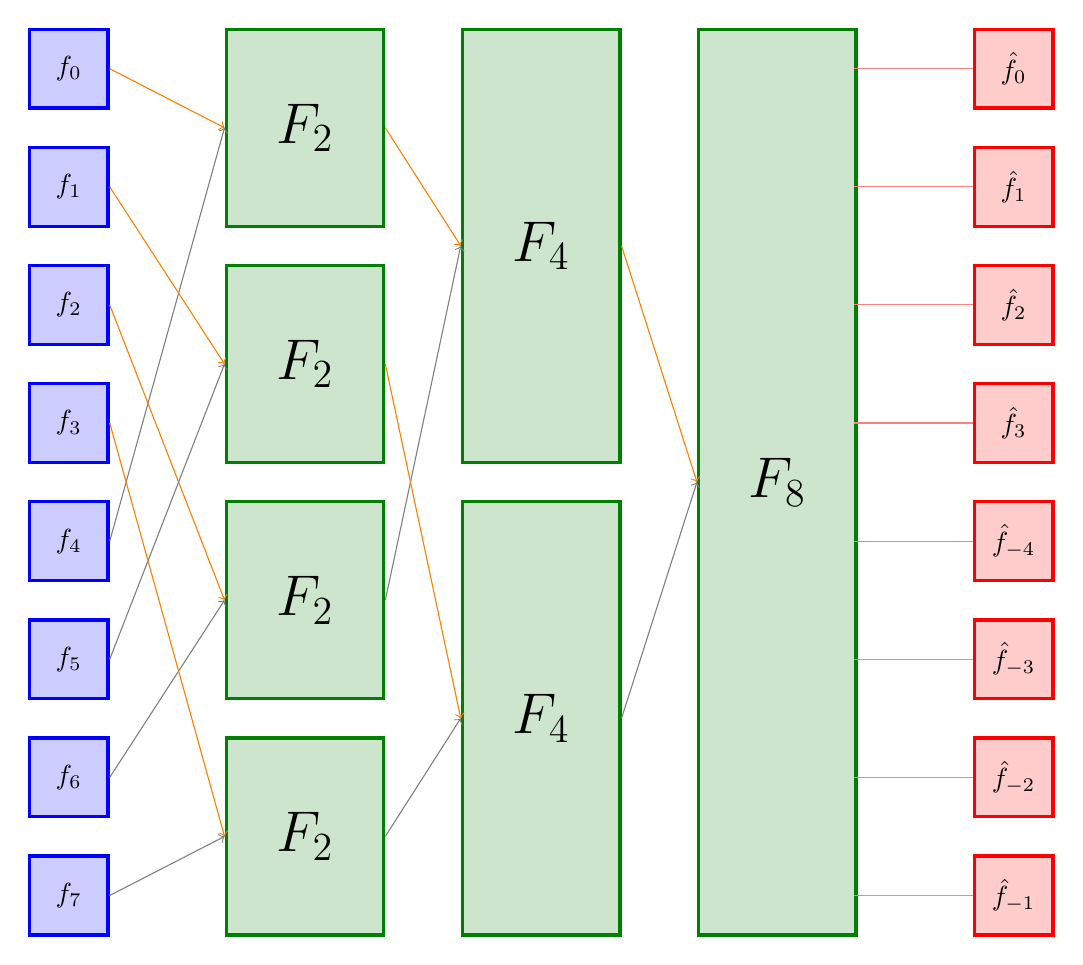
\begin{tikzpicture}[squarednode/.style={rectangle, draw=blue!, fill=blue!20, very thick, align=center, minimum size=10mm},
    squaredrnode/.style={rectangle, draw=red!, fill=red!20, very thick, align=center, minimum size=10mm},
    rectnode/.style={rectangle, draw=Green!, fill=Green!20, very thick, align=center, minimum size=20mm}]
    \node[squarednode] at (0,0) (f0) {$f_0$};
    \node[squarednode] at (0,-1.5) (f1) {$f_1$};
    \node[squarednode] at (0,-3) (f2) {$f_2$};
    \node[squarednode] at (0,-4.5) (f3) {$f_3$};
    \node[squarednode] at (0,-6) (f4) {$f_4$};
    \node[squarednode] at (0,-7.5) (f5) {$f_5$};
    \node[squarednode] at (0,-9) (f6) {$f_6$};
    \node[squarednode] at (0,-10.5) (f7) {$f_7$};
    \node[rectnode, minimum height=25mm] at (3, -0.75) (F21) {\huge $F_2$};
    \node[rectnode, minimum height=25mm] at (3, -3.75) (F22) {\huge $F_2$};
    \node[rectnode, minimum height=25mm] at (3, -6.75) (F23) {\huge $F_2$};
    \node[rectnode, minimum height=25mm] at (3, -9.75) (F24) {\huge $F_2$};
    \draw[orange, ->] (f0.east) -- (F21.west);
    \draw[gray, ->] (f4.east) -- (F21.west);
    \draw[orange, ->] (f2.east) -- (F23.west);
    \draw[gray, ->] (f6.east) -- (F23.west);
    \draw[orange, ->] (f1.east) -- (F22.west);
    \draw[gray, ->] (f5.east) -- (F22.west);
    \draw[orange, ->] (f3.east) -- (F24.west);
    \draw[gray, ->] (f7.east) -- (F24.west);
    \node[rectnode, minimum height=55mm] at (6, -2.25) (F41) {\huge $F_4$};
    \node[rectnode, minimum height=55mm] at (6, -8.25) (F42) {\huge $F_4$};
    \draw[orange, ->] (F21.east) -- (F41.west);
    \draw[gray, ->] (F23.east) -- (F41.west);
    \draw[orange, ->] (F22.east) -- (F42.west);
    \draw[gray, ->] (F24.east) -- (F42.west);
    \node[rectnode, minimum height=115mm] at (9, -5.25) (F8) {\huge $F_8$};
    \draw[orange, ->] (F41.east) -- (F8.west);
    \draw[gray, ->] (F42.east) -- (F8.west);
    \node[squaredrnode] at (12,0) (fh0) {$\hat{f}_0$};
    \node[squaredrnode] at (12,-1.5) (fh1) {$\hat{f}_1$};
    \node[squaredrnode] at (12,-3) (fh2) {$\hat{f}_2$};
    \node[squaredrnode] at (12,-4.5) (fh3) {$\hat{f}_3$};
    \node[squaredrnode] at (12,-6) (fh4) {$\hat{f}_{-4}$};
    \node[squaredrnode] at (12,-7.5) (fh5) {$\hat{f}_{-3}$};
    \node[squaredrnode] at (12,-9) (fh6) {$\hat{f}_{-2}$};
    \node[squaredrnode] at (12,-10.5) (fh7) {$\hat{f}_{-1}$};
    \draw[red!50] (fh0.west) --++ (-1.5,0);
    \draw[red!50] (fh1.west) --++ (-1.5,0);
    \draw[red!50] (fh2.west) --++ (-1.5,0);
    \draw[red!50] (fh3.west) --++ (-1.5,0);
    \draw[red!50] (fh4.west) --++ (-1.5,0);
    \draw[red!50] (fh5.west) --++ (-1.5,0);
    \draw[red!50] (fh6.west) --++ (-1.5,0);
    \draw[red!50] (fh7.west) --++ (-1.5,0);
    \end{tikzpicture}
    \caption{A schematic diagram outlining the principle of FFT.}
    \label{fig:FFT}
\end{figure}
\end{landscape}

\section{Python Programming and Earth System Applications}

Since in practice the time-series to be processed are often very long, it is impossible to do DFT/FFT manually and we will combine the application part with the programming tutorial into one single section. We will use the Niño 3.4 SST Index which is an indicator of the ENSO phenomenon discussed in Section \ref{section:EOF} for demonstration. Now, download the data file from \href{https://psl.noaa.gov/data/timeseries/month/data/nino34.long.anom.csv}{https://psl.noaa.gov/data/timeseries/month/data/nino34.long.anom.csv} and use the following code to read the time-series.
\begin{lstlisting}
import numpy as np
import pandas as pd

Nino34 = pd.read_csv("nino34.long.anom.csv", header=0, names=["Date", "Nino34"])
print(Nino34)    
\end{lstlisting}
Next, import the required functions from the \verb|scipy.fft| module and apply FFT on the Niño 3.4 time-series over the 120 years time period of 1901-2020.
\begin{lstlisting}
from scipy.fft import fft, fftfreq, fftshift

Nino34_120yrs = Nino34[(Nino34["Date"] >= "1901-01-01") & (Nino34["Date"] <= "2020-12-31")]
print(Nino34_120yrs)

Nino34_fft = fft(Nino34_120yrs["Nino34"].values) 
\end{lstlisting}
Compute the power spectrum by multiplying the FFT-transformed data by its complex conjugate.
\begin{lstlisting}
Nino34_power = np.real(Nino34_fft*np.conjugate(Nino34_fft)) # Call the function np.real to remove negligible imaginary parts due to round-off error. Alternatively, write np.abs(Nino34_fft)**2.
\end{lstlisting}
Use the \verb|fftfreq| function to produce the frequency and period bins.
\begin{lstlisting}
Nino34_freq = fftfreq(len(Nino34_power), 1/12) # 1 month = 1/12 yrs
Nino34_period = 1/Nino34_freq
\end{lstlisting}
Finally, we can plot the power spectrum as follows.
\begin{lstlisting}
import matplotlib.pyplot as plt

def reciprocal(x): # Function to transform between frequency and period for the secondary axis.
    return(1/x)

plt.plot(Nino34_freq[:len(Nino34_power)//2], Nino34_power[:len(Nino34_power)//2])
plt.xlabel("Frequency (per yr)")
period_ax = plt.gca().secondary_xaxis('top', functions=(reciprocal, reciprocal))
plt.xlim([1/60,1])
period_ax.set_ticks([1,2,3,4,5,6,8,12])
period_ax.set_xlabel("Period (yr)")
plt.savefig("NinoFFT", dpi=300, bbox_inches="tight")
\end{lstlisting}
\begin{center}
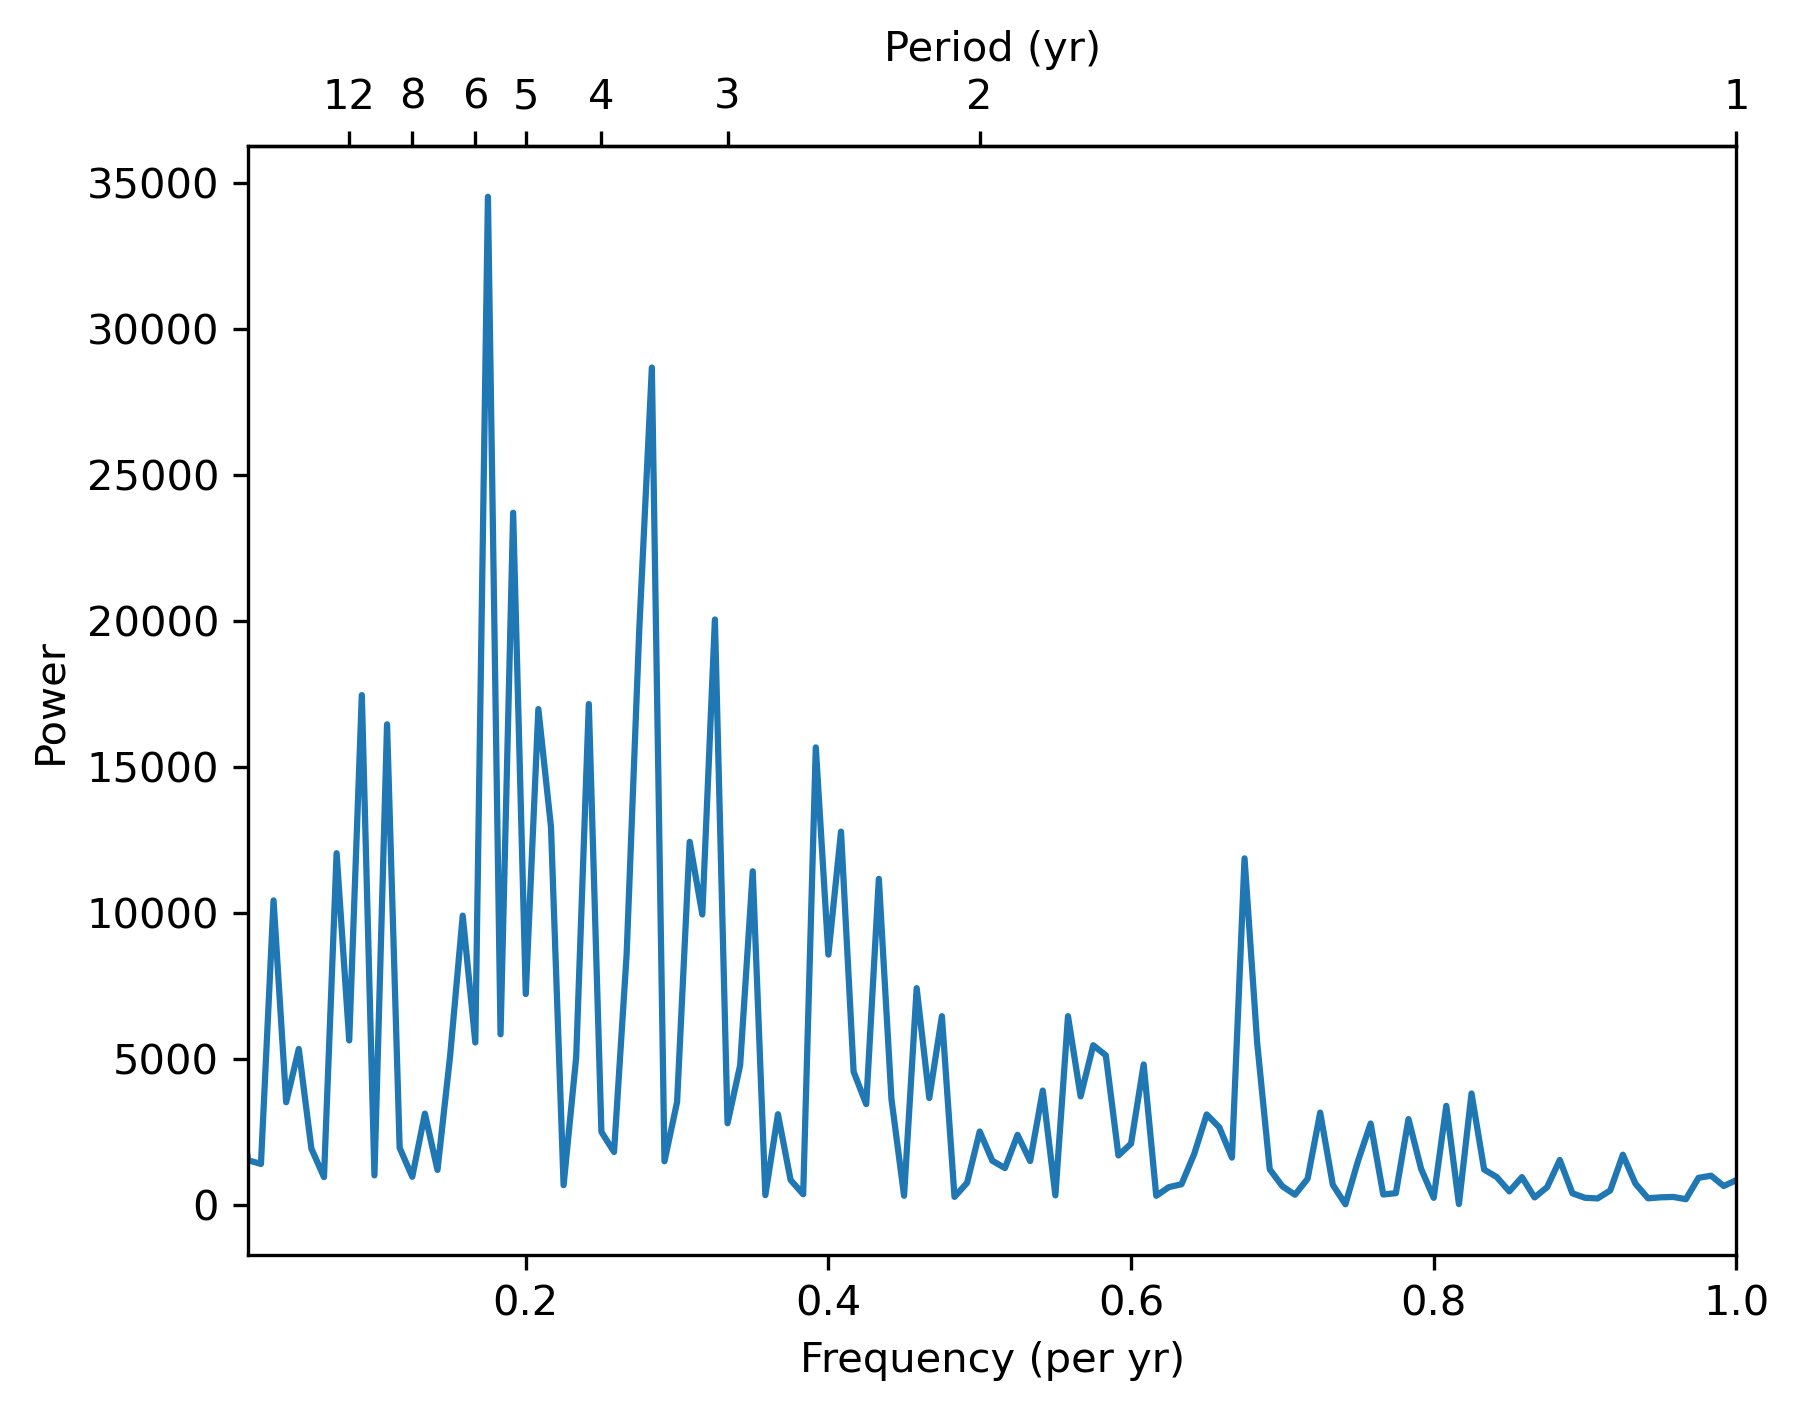
\includegraphics[scale=0.75]{graphics/NinoFFT.png}
\end{center}
It can be seen that the strongest signals are located over the periods from $2.5$ to $7$ years, which coincides with the typical time scale of ENSO. We can carry out a simple filtering to extract the Niño 3.4 signals corresponding to ENSO by zeroing out the FFT array at all other frequencies and then applying an inverse FFT: 
\begin{lstlisting}
from scipy.fft import ifft

Nino34_fft_ENSO = np.copy(Nino34_fft)
Nino34_fft_ENSO[~((2.5 <= np.abs(Nino34_period)) & (np.abs(Nino34_period) <= 7))] = 0
Nino34_ENSO = np.real(ifft(Nino34_fft_ENSO))
\end{lstlisting}
Let's make a plot to compare the filtered time-series with the original one.
\begin{lstlisting}
plt.plot(Nino34_120yrs["Date"], Nino34_120yrs["Nino34"].values, label="raw")
plt.plot(Nino34_120yrs["Date"], Nino34_ENSO, label="FFT-filtered")
plt.xticks(np.arange(0,len(Nino34_120yrs["Date"]), 60), rotation=20)
plt.xlim(["1981-01-01", "2020-12-31"])
plt.xlabel("Date")
plt.ylabel("Nino 3.4 Index")
plt.legend()
plt.title("ENSO-filtered Nino 3.4 Time-series")
plt.savefig("NinoENSOFilter", dpi=300, bbox_inches="tight")
\end{lstlisting}
However, note that this "zeroing-out" filtering method is not a very good idea to be implemented in practice and we do it here only for a heuristic purpose. For more information, search about the \textit{"Gibbs Phenomenon"} and also read the comprehensive discussion in   \href{https://stackoverflow.com/questions/31256252/why-does-numpy-linalg-solve-offer-more-precise-matrix-inversions-than-numpy-li}{this DSP StackExchange post} (6220).
\begin{center}
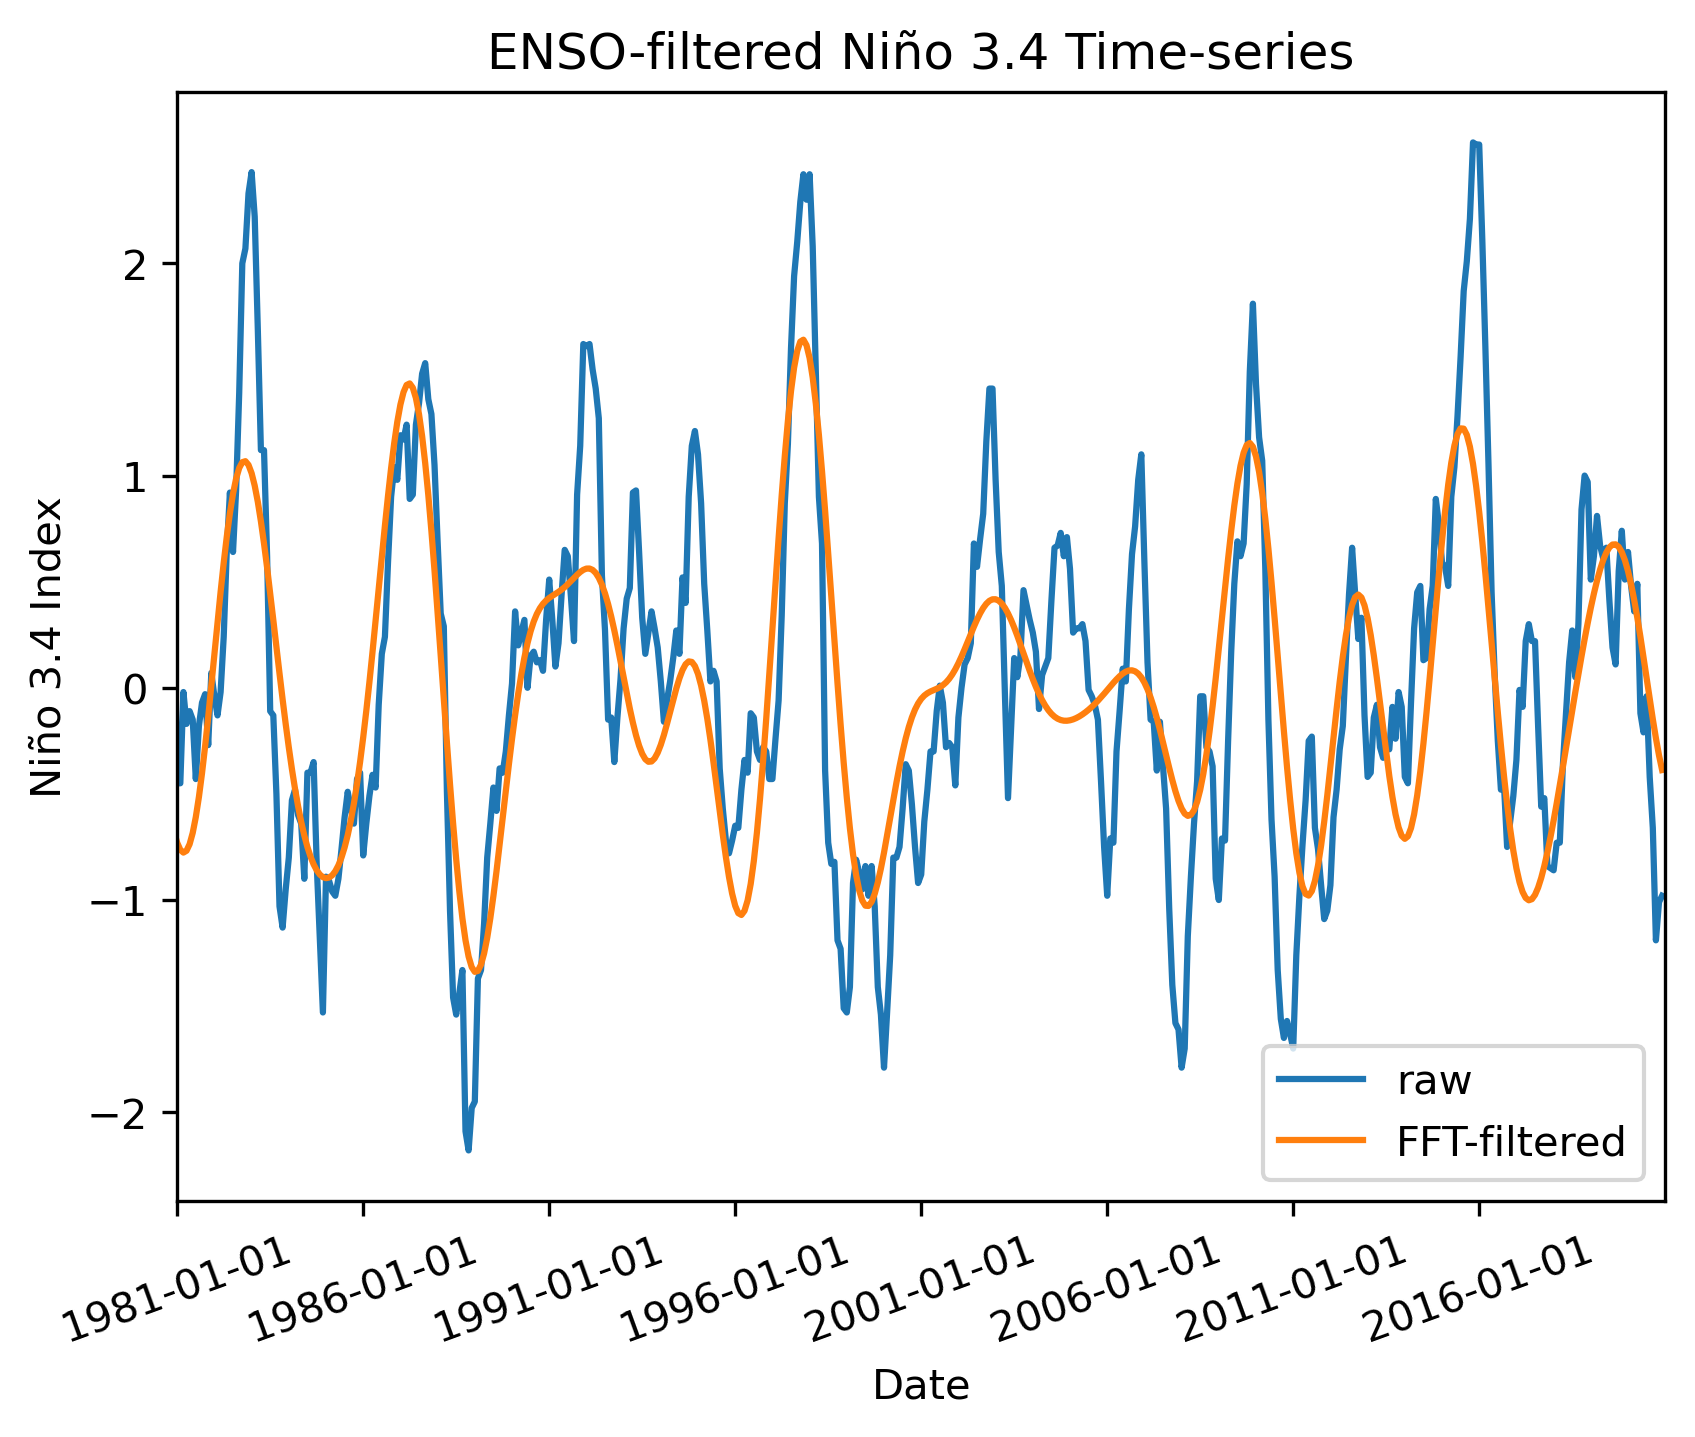
\includegraphics[scale=0.8]{graphics/NinoENSOFilter.png}
\end{center}


\section{Exercise}
\begin{Exercise}
Compute the Discrete Fourier Transform for the following data.
\begin{center}
\begin{tabular}{|c|c|c|c|c|c|c|}
\hline
unit time & 0 & 1 & 2 & 3 & 4 \\
\hline
f(t) & 4.5 & 6.2 & 7.8 & 1.1 & 3.4  \\
\hline
unit time & 5 & 6 & 7 & 8 & 9 \\
\hline
f(t) & 2.5 & 3.6 & 5.9 & 2.9 & 6.0\\
\hline
\end{tabular}
\end{center}
Find the amplitude/power and phase of the sinusoidal wave signal corresponding to the third frequency bin, i.e.\ with an angular frequency of $\omega = \frac{2\pi(3)}{10}$. 
\end{Exercise}

\begin{Exercise}
Download an \href{https://cds.climate.copernicus.eu/datasets/reanalysis-era5-single-levels?tab=download}{ERA5 Temperature dataset} over any time period of $20$ years. Select any location as you like, and extract the temperature time-series there. Apply DFT on the time series, and identify any dominant frequency or period with a tall power. Explain the peaks with Earth Science knowledge.
\end{Exercise}

\begin{Exercise}
Perform DFT on the time-series for the two MJO EOF modes derived in Exercise (\ref{ex:MJO}) and deduce the characteristic time scale of MJO by plotting the power spectrum against periods.
\end{Exercise}

\begin{Exercise}
Find the circular convolution of two time-series $f(t) = (1,4,2,4, \\ 3,0,-1,2)$ and $g(t) = (2,3,-2,1,-1,0,4,3)$ by definition, as well as via the Convolution Theorem to check the consistency.
\end{Exercise}

\begin{Exercise}
Write your own FFT function in Python and compare with the one in the \verb|scipy.fft| library by testing them on any time-series.
\end{Exercise}